%% Chapter Template
%
\chapter{Animation for Data Reshaping} \label{c5} % Main chapter title

In this chapter we will discuss how we use animations to expression data reshaping.

\section{Long to Wide (Spread)}

\subsection{Logic of Long to Wide}
The logic of the long to wide transformation in the \texttt{spread} function of \textbf{tidyr} is to use the \texttt{key} and \texttt{value} column. Note that the \texttt{key} does not have the same definition as the key column in data joins. The \texttt{key} here is the column the user wishes to use to spread out to multiple columns and the \texttt{value} is the column that contains their values.

\subsection{Long to Wide Animation}
Before the animation starts, we tell the user that we will be using a old column from the original table given by the user to create new columns in the resulted table by using a message. Here we will use the old column Subject to spread out (create) two columns English and Maths.

We then move elements English and Maths from the original table up to the message because we want the user to know that these are the columns we will be using during the animation (Fig.~\ref{fig:spread1}). We use a table cell like design for this word within the sentence because we want the user to know that we are referring to a certain element in a particular table. We will use this table cell technique often through out the reshaping animation.

\begin{figure}[H]
    % \centering
    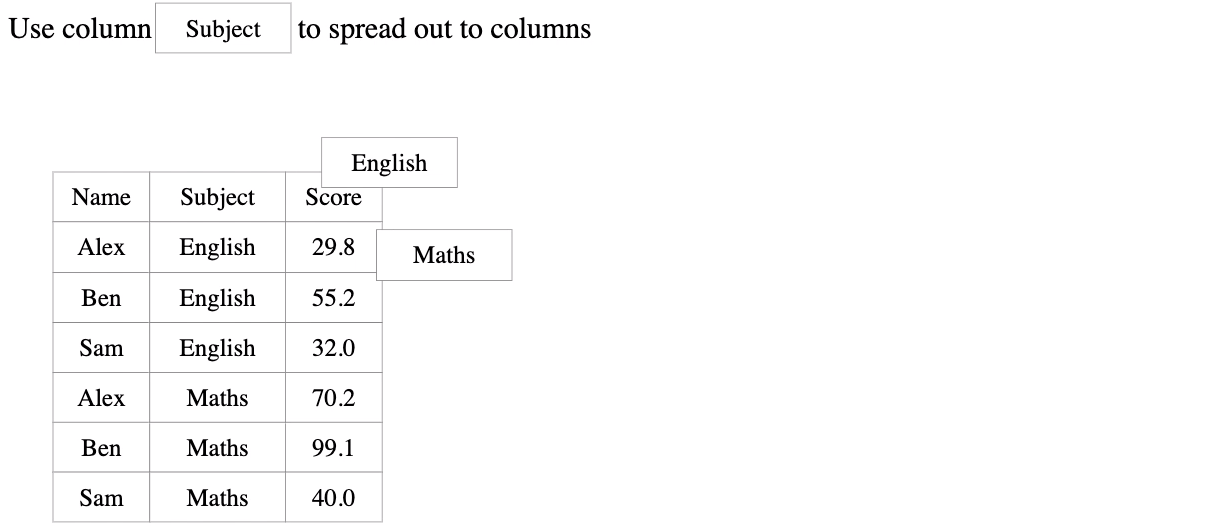
\includegraphics[scale = 0.35]{Masters-Thesis/img/spread1.png}
    \caption{Long to Wide step 1}
    \label{fig:spread1}
\end{figure}

Second, we show another message informing the user that we will use the values in the Score column for this transformation (Fig.~\ref{fig:spread2}). Again, the word Score is in a table cell like design. 
\begin{figure}[H]
    % \centering
    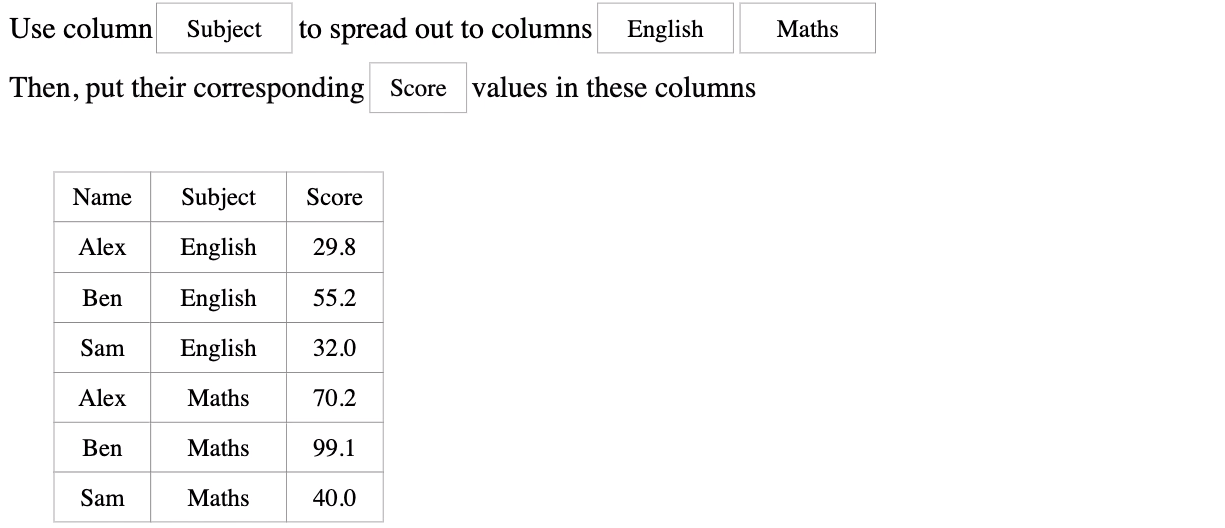
\includegraphics[scale = 0.35]{Masters-Thesis/img/spread2.png}
    \caption{Long to Wide step 2}
    \label{fig:spread2}
\end{figure}


Third, we show the structure of the resulted table. This is to give the user an idea of what the resulted table will look like. This table is currently empty and only contain column names, these empty cells will be filled in though out the animation (Fig.~\ref{fig:spread3}). 
\begin{figure}[H]
    % \centering
    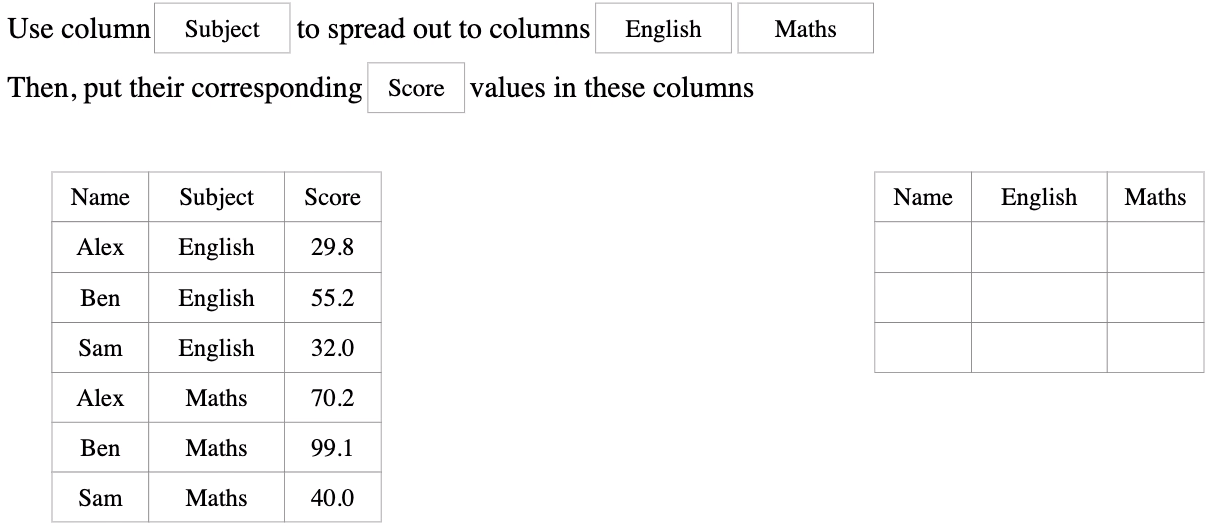
\includegraphics[scale = 0.35]{Masters-Thesis/img/spread3.png}
    \caption{Long to Wide step 3}
    \label{fig:spread3}
\end{figure}
\newpage

Fourth, we fade out the tables and the text in the background. Then we show a message informing the user that the animation will now start and that the first step is to move across unique values from the column that is neither the key or value across to the resulted table (Fig.~\ref{fig:spread4}). For example, here we show a message "Move across unique values from Name". We fade out the background to allow the user to focus on this message.
\begin{figure}[H]
    % \centering
    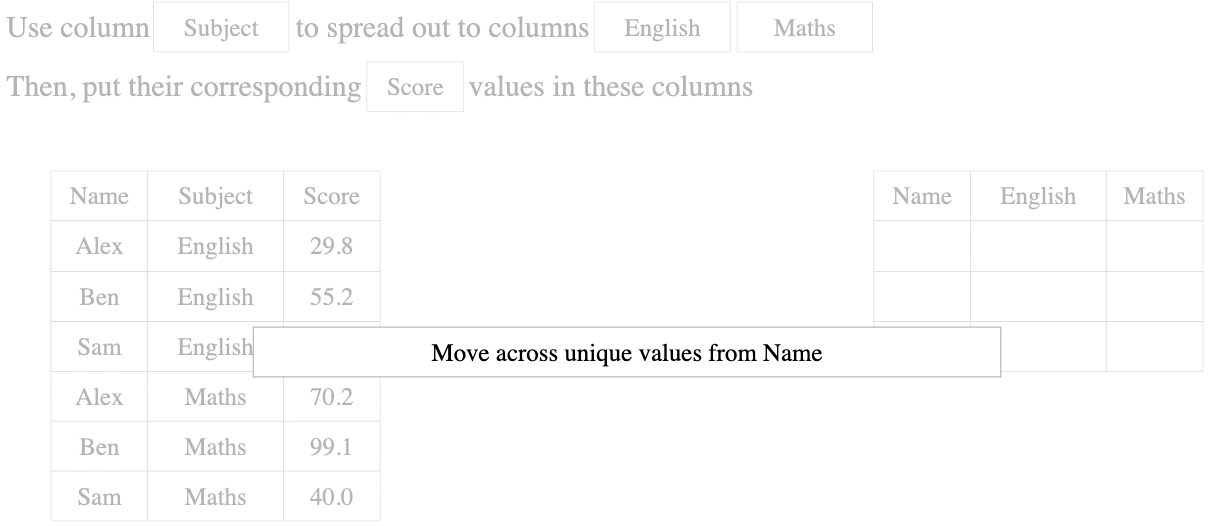
\includegraphics[scale = 0.35]{Masters-Thesis/img/spread4.png}
    \caption{Long to Wide step 4}
    \label{fig:spread4}
\end{figure}

Fifth, we flash the unique elements in the Name column, to catch the users attention Fig.~\ref{fig:spread5}).
\begin{figure}[H]
    % \centering
    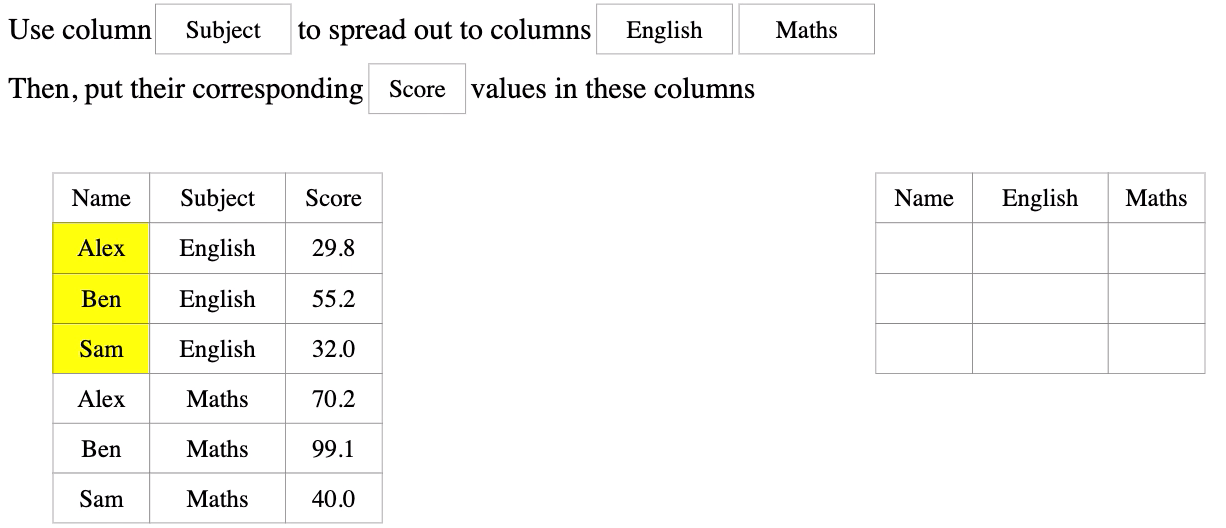
\includegraphics[scale = 0.35]{Masters-Thesis/img/spread5.png}
    \caption{Long to Wide step 5}
    \label{fig:spread5}
\end{figure}
\newpage
Sixth, we move the unique names over to the resulted table Fig.~\ref{fig:spread6}, caught mid-move).
\begin{figure}[H]
    % \centering
    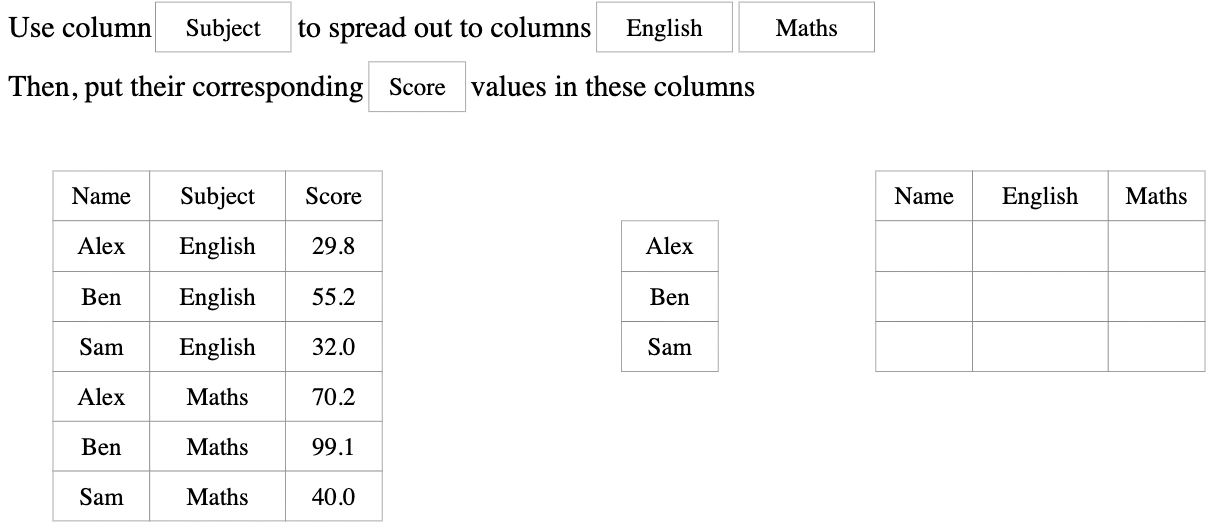
\includegraphics[scale = 0.35]{Masters-Thesis/img/spread6.png}
    \caption{Long to Wide step 6}
    \label{fig:spread6}
\end{figure}

Next, we flash the first set of unique row in the original table. Here, it is Alex and English in the original table. To catch the users attention to this row, the elements containing these values in the resulted table will also flash (Fig.~\ref{fig:spread7}). Here, we want the user to understand the relationship between the two tables. 
\begin{figure}[H]
    % \centering
    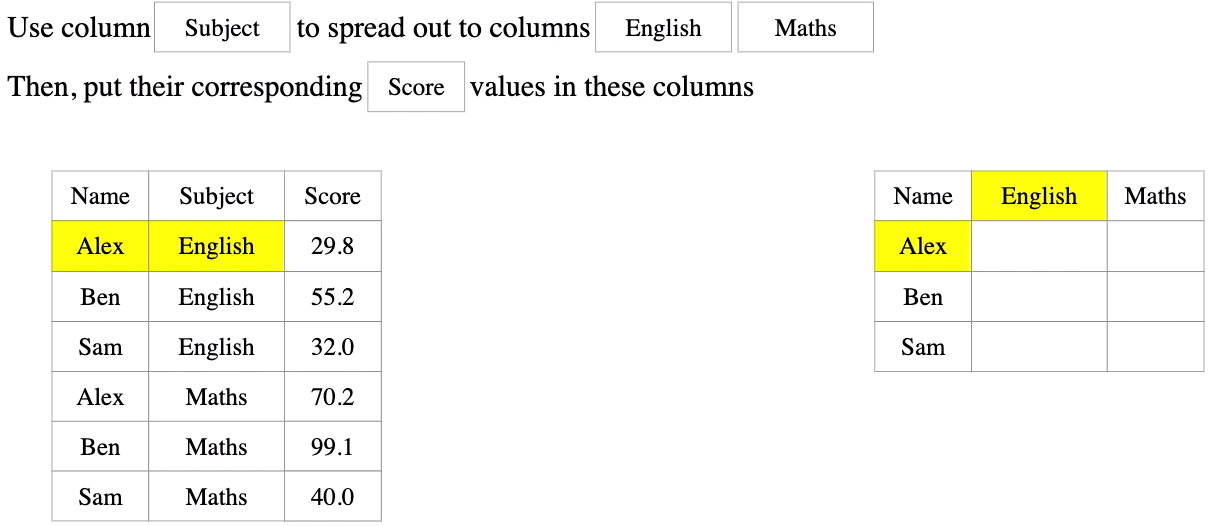
\includegraphics[scale = 0.35]{Masters-Thesis/img/spread7.png}
    \caption{Long to Wide step 7}
    \label{fig:spread7}
\end{figure}

\newpage
The values of the previously flashed rows will then move into its corresponding location in the resulted table. The correct location for this cell will be the intersect of the two flashed cells in the result table (Fig.~\ref{fig:spread8}, caught mid-move). The animation continues sequentially down the rows of the original table. 
\begin{figure}[H]
    % \centering
    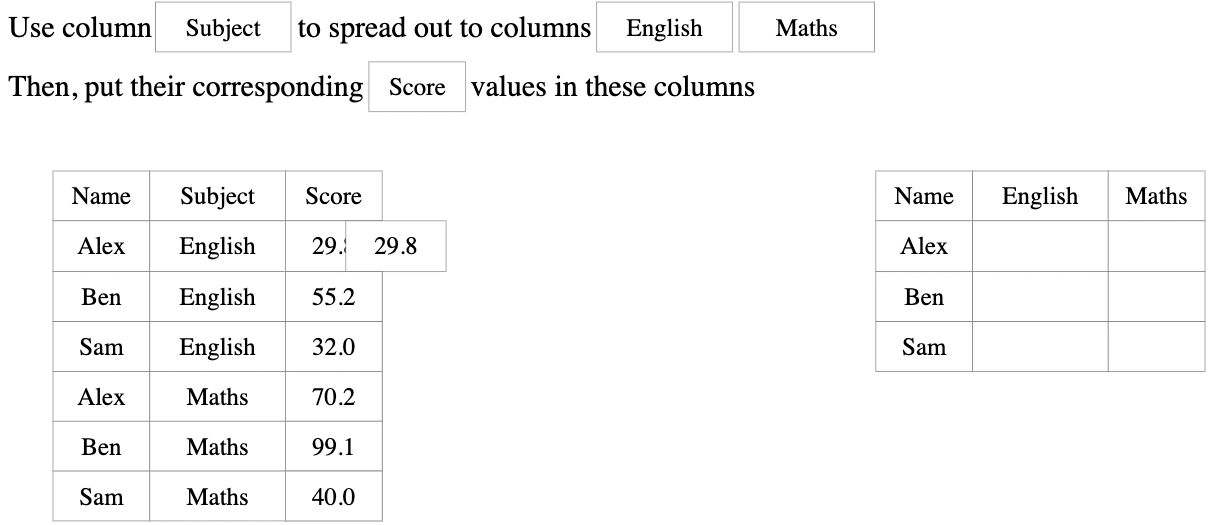
\includegraphics[scale = 0.35]{Masters-Thesis/img/spread8.png}
    \caption{Long to Wide step 8}
    \label{fig:spread8}
\end{figure}

We then do the same for Maths after we are finished with English (Fig.~\ref{fig:spread9}).
\begin{figure}[H]
    % \centering
    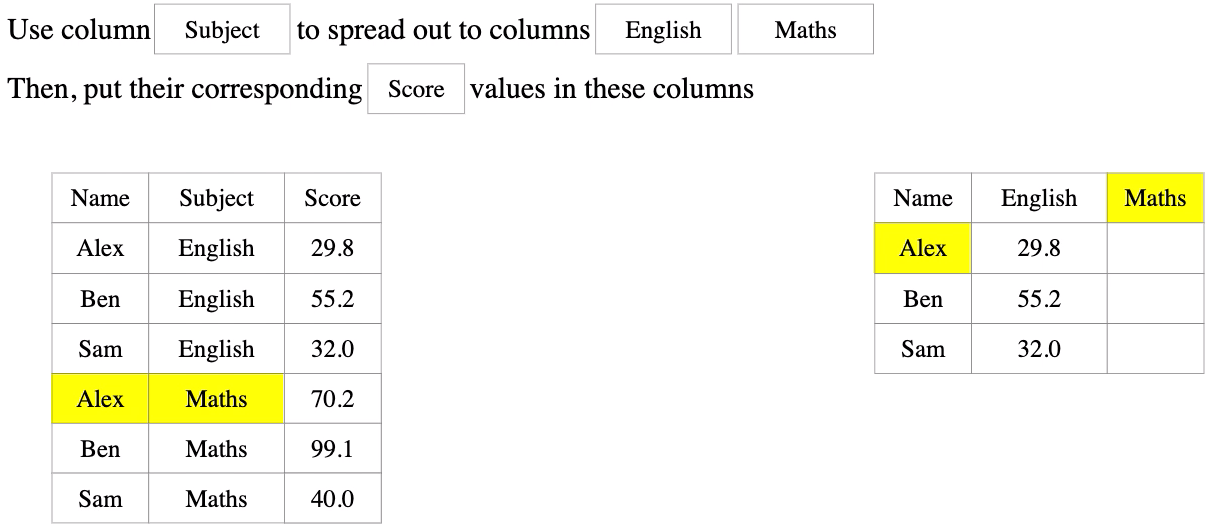
\includegraphics[scale = 0.35]{Masters-Thesis/img/spread9.png}
    \caption{Long to Wide step 9}
    \label{fig:spread9}
\end{figure}

\newpage
Lastly, when the animation finishes, the animation will stop (Fig.~\ref{fig:spread10}).
\begin{figure}[H]
    % \centering
    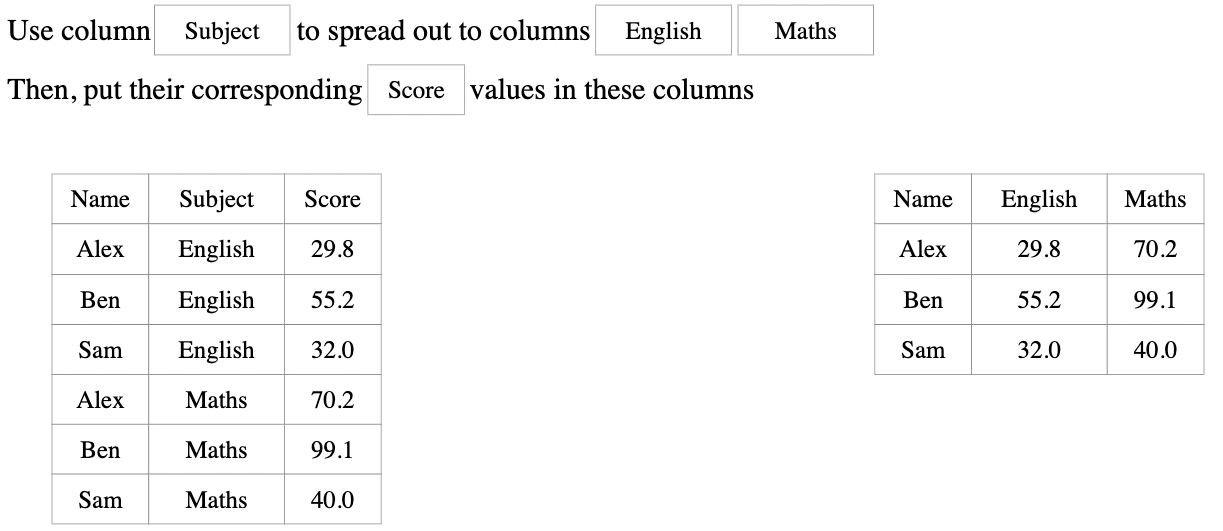
\includegraphics[scale = 0.35]{Masters-Thesis/img/spread10.png}
    \caption{Long to Wide step 10}
    \label{fig:spread10}
\end{figure}


\section{Wide to Long (Gather)}
\subsection{Logic of Wide to Long}
The logic of the wide to long transformation in the \texttt{gather} function of \textbf{tidyr} is to use the \texttt{key} and \texttt{value} column, this is the same as \texttt{gather}. However, the meaning of the \texttt{key} and \texttt{value} is different. Here, \texttt{key} is the new column name the user wishes to use to contain old column names. The \texttt{value} is the new column name to contain the old column values. An additional argument is required by \texttt{gather}, the user will also need to provide the columns they wish to transform the data on. 

\subsection{Wide to Long Animation}
Before the animation starts, we tell the user that we will create a new column to contain old column names by using a message. Here we will create a new column named Subject to contain the old column names English and Maths.

We then move elements English and Maths from the original table up to the message because we want the user to know that these are the columns we will be using during the animation (Fig.~\ref{fig:gather1}).
\begin{figure}[H]
    % \centering
    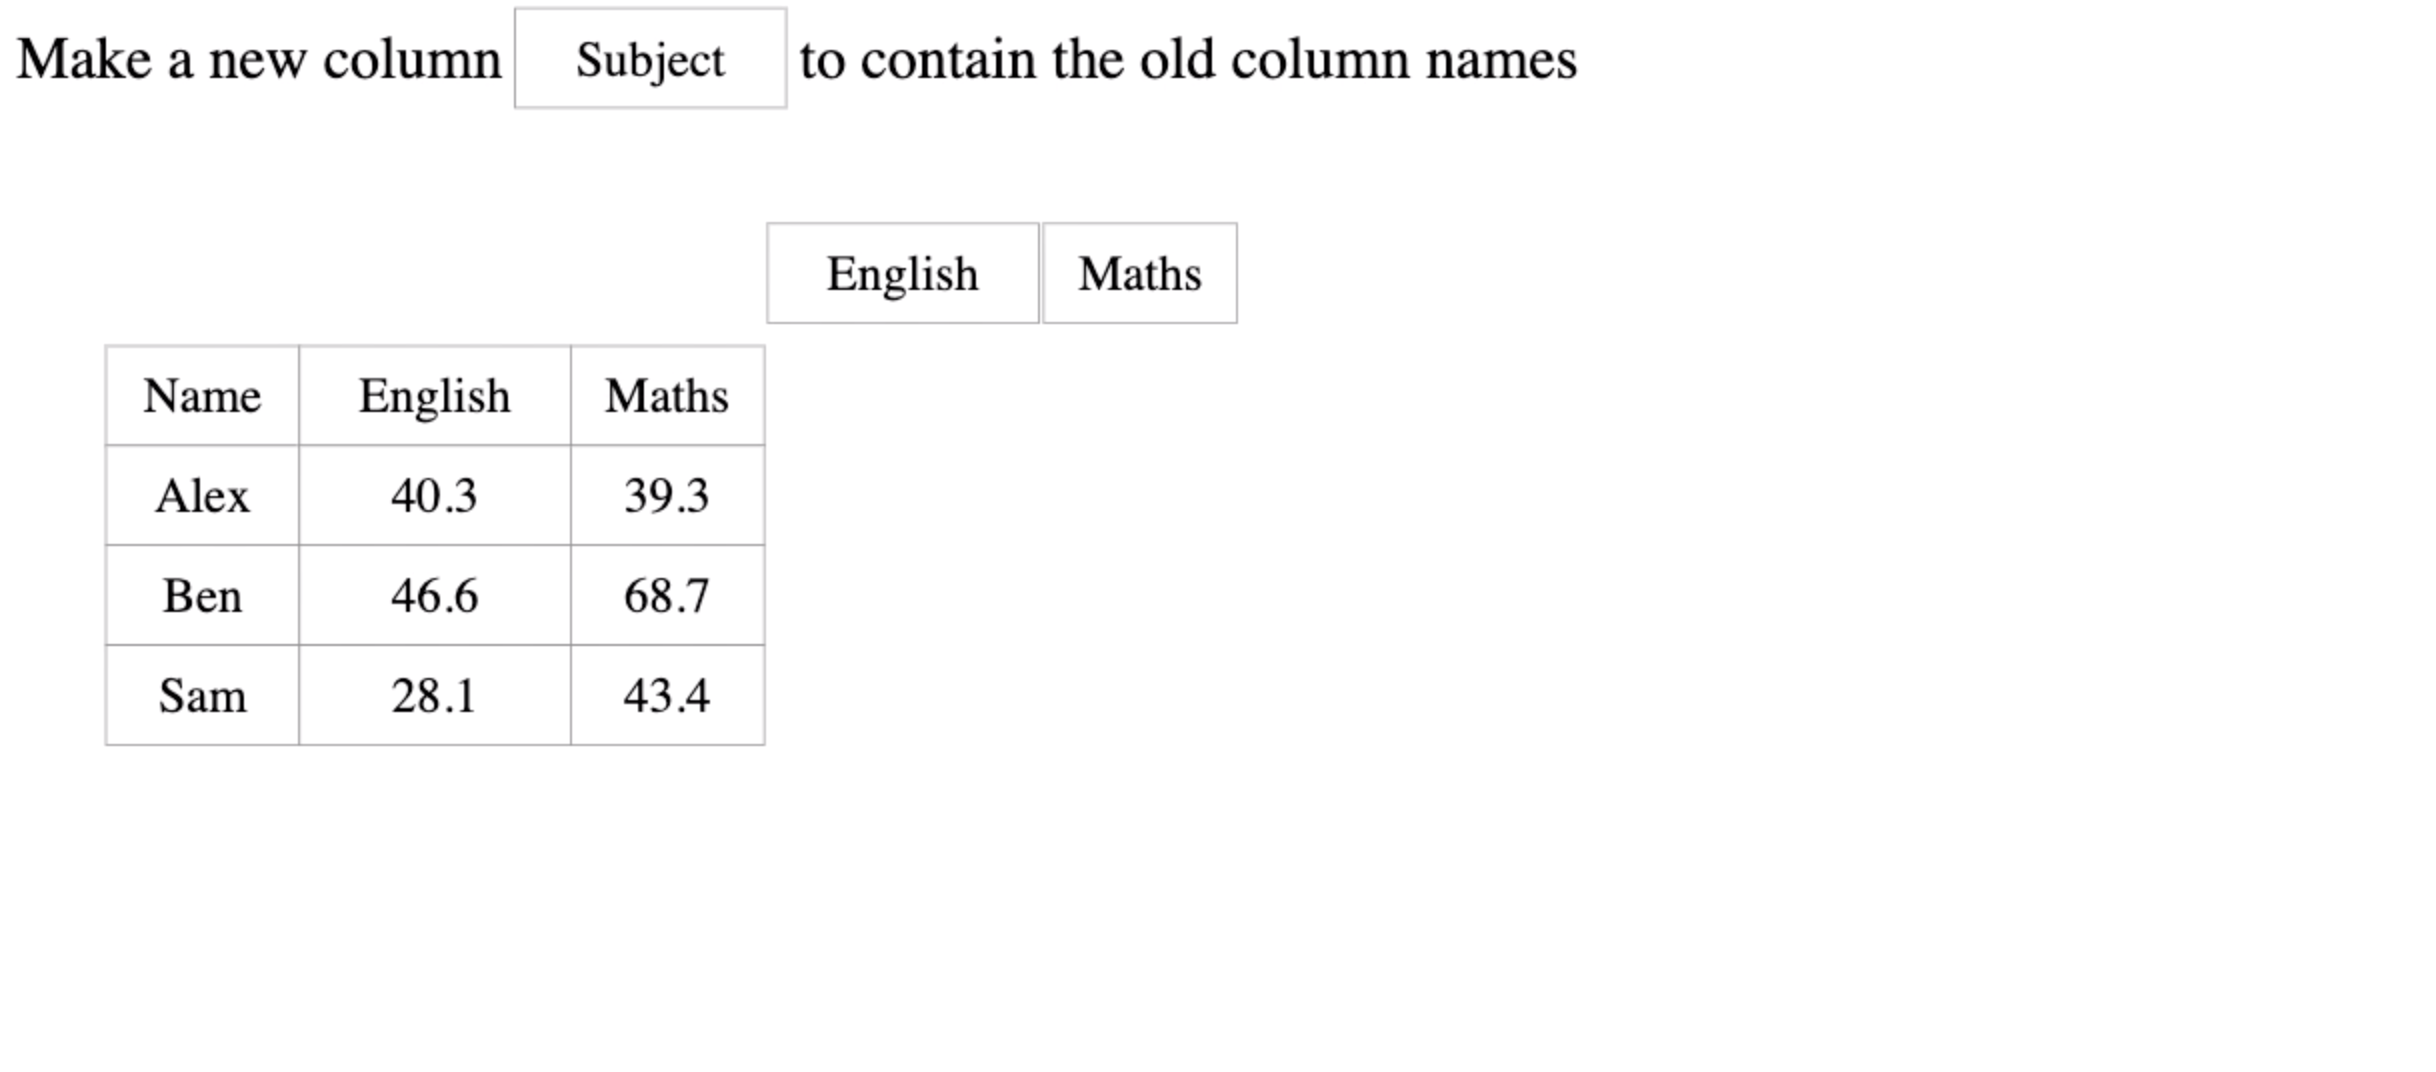
\includegraphics[scale = 0.35]{Masters-Thesis/img/gather1.png}
    \caption{Wide to Long step 1}
    \label{fig:gather1}
\end{figure}

Second, we show another message informing the user that we will create another new column to contain the old column values. Here we will create a new column in the resulted table called Score (Fig.~\ref{fig:gather2}).
\begin{figure}[H]
    % \centering
    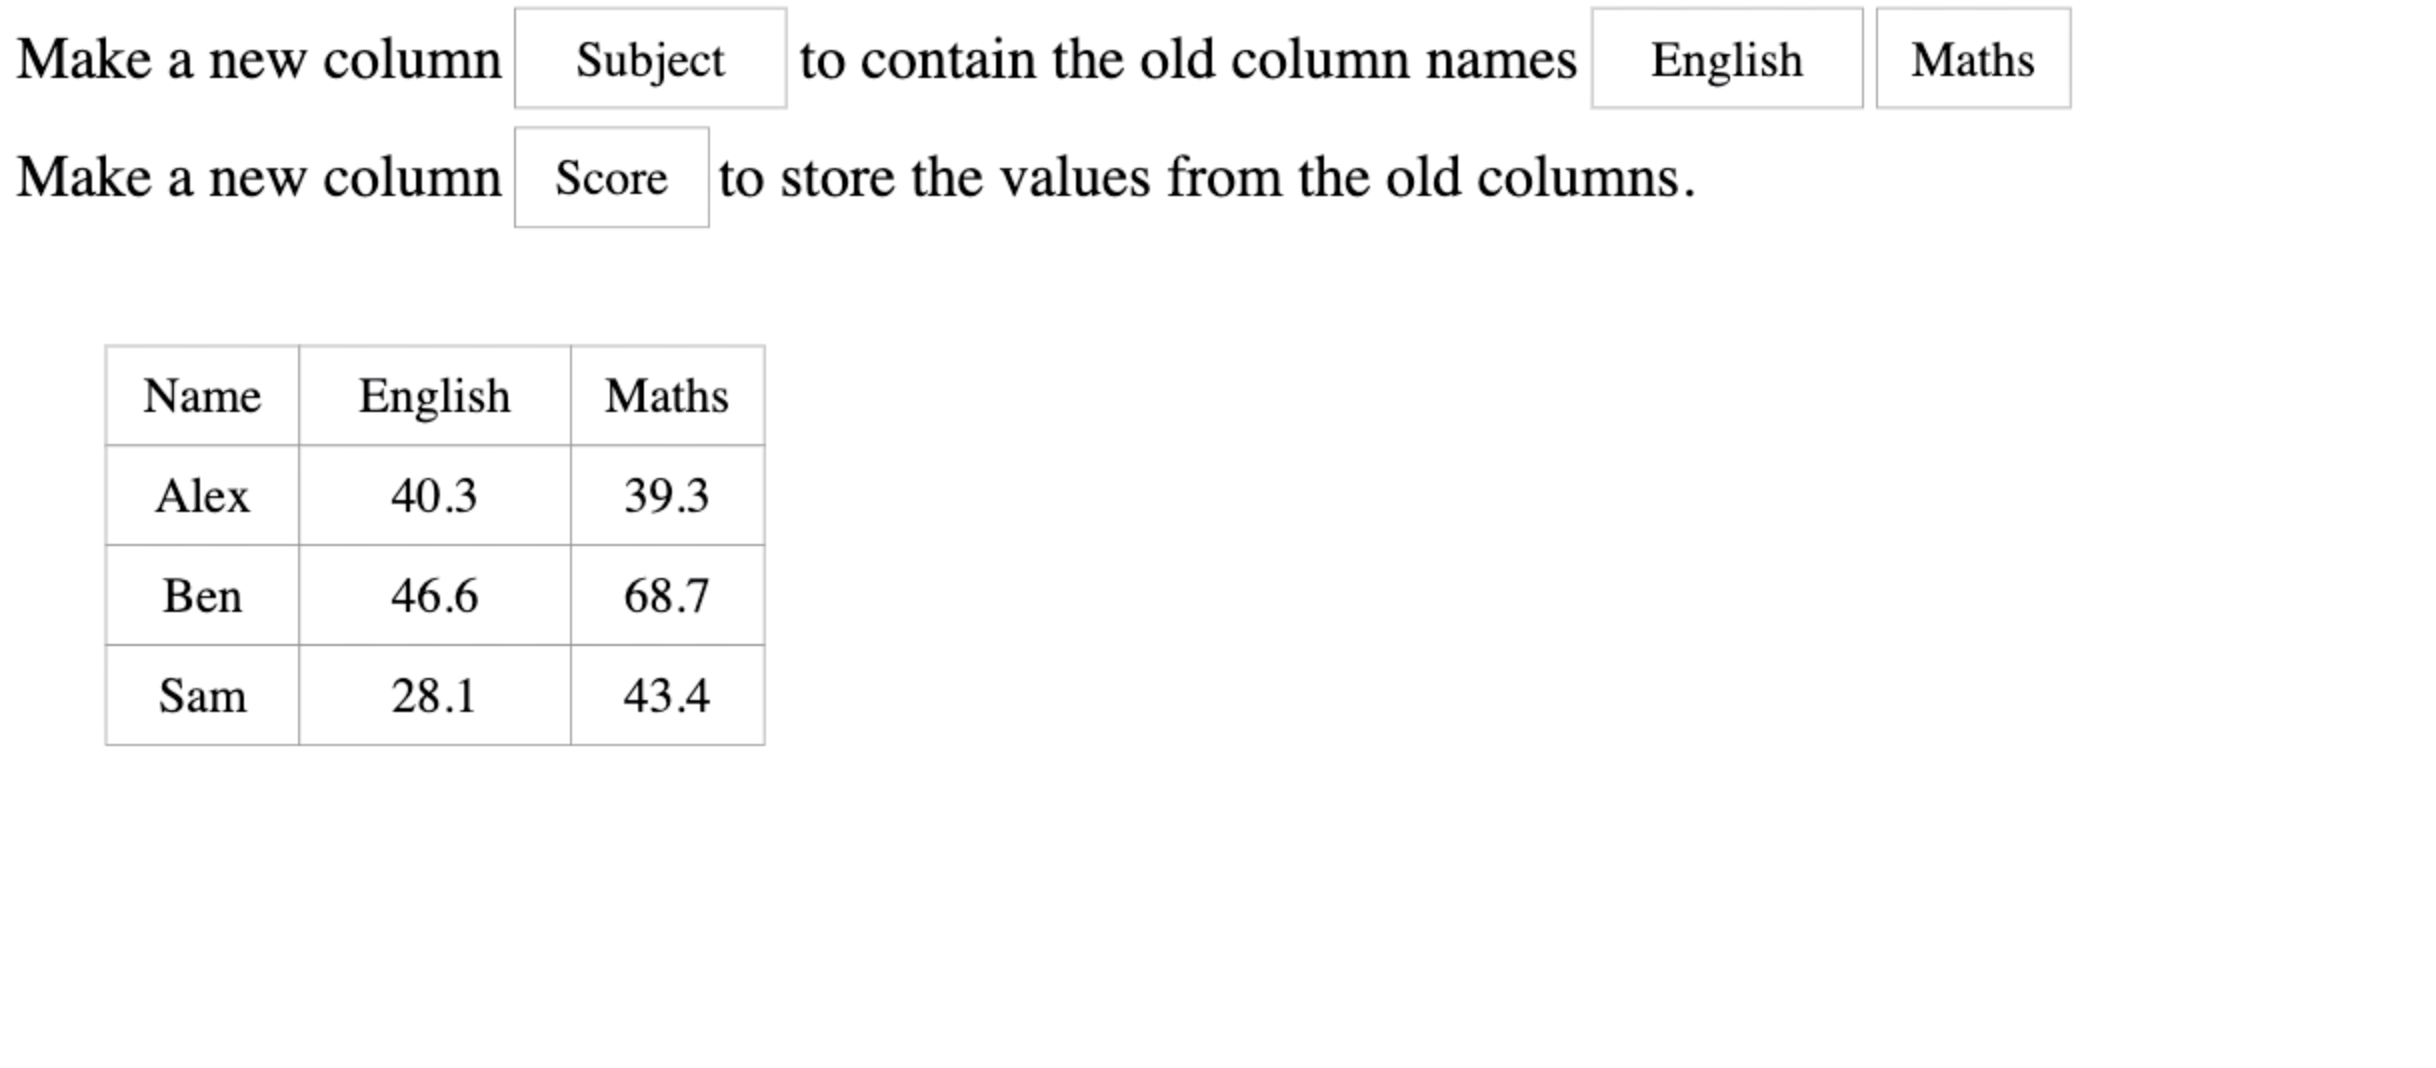
\includegraphics[scale = 0.35]{Masters-Thesis/img/gather2.png}
    \caption{Wide to Long step 2}
    \label{fig:gather2}
\end{figure}

\newpage
Third, we show the structure of the resulted table. This is to give the user an idea of what the resulted table will look like. This table is currently empty and only contain column names, these empty cells will be filled in though out the animation (Fig.~\ref{fig:gather3}).
\begin{figure}[H]
    % \centering
    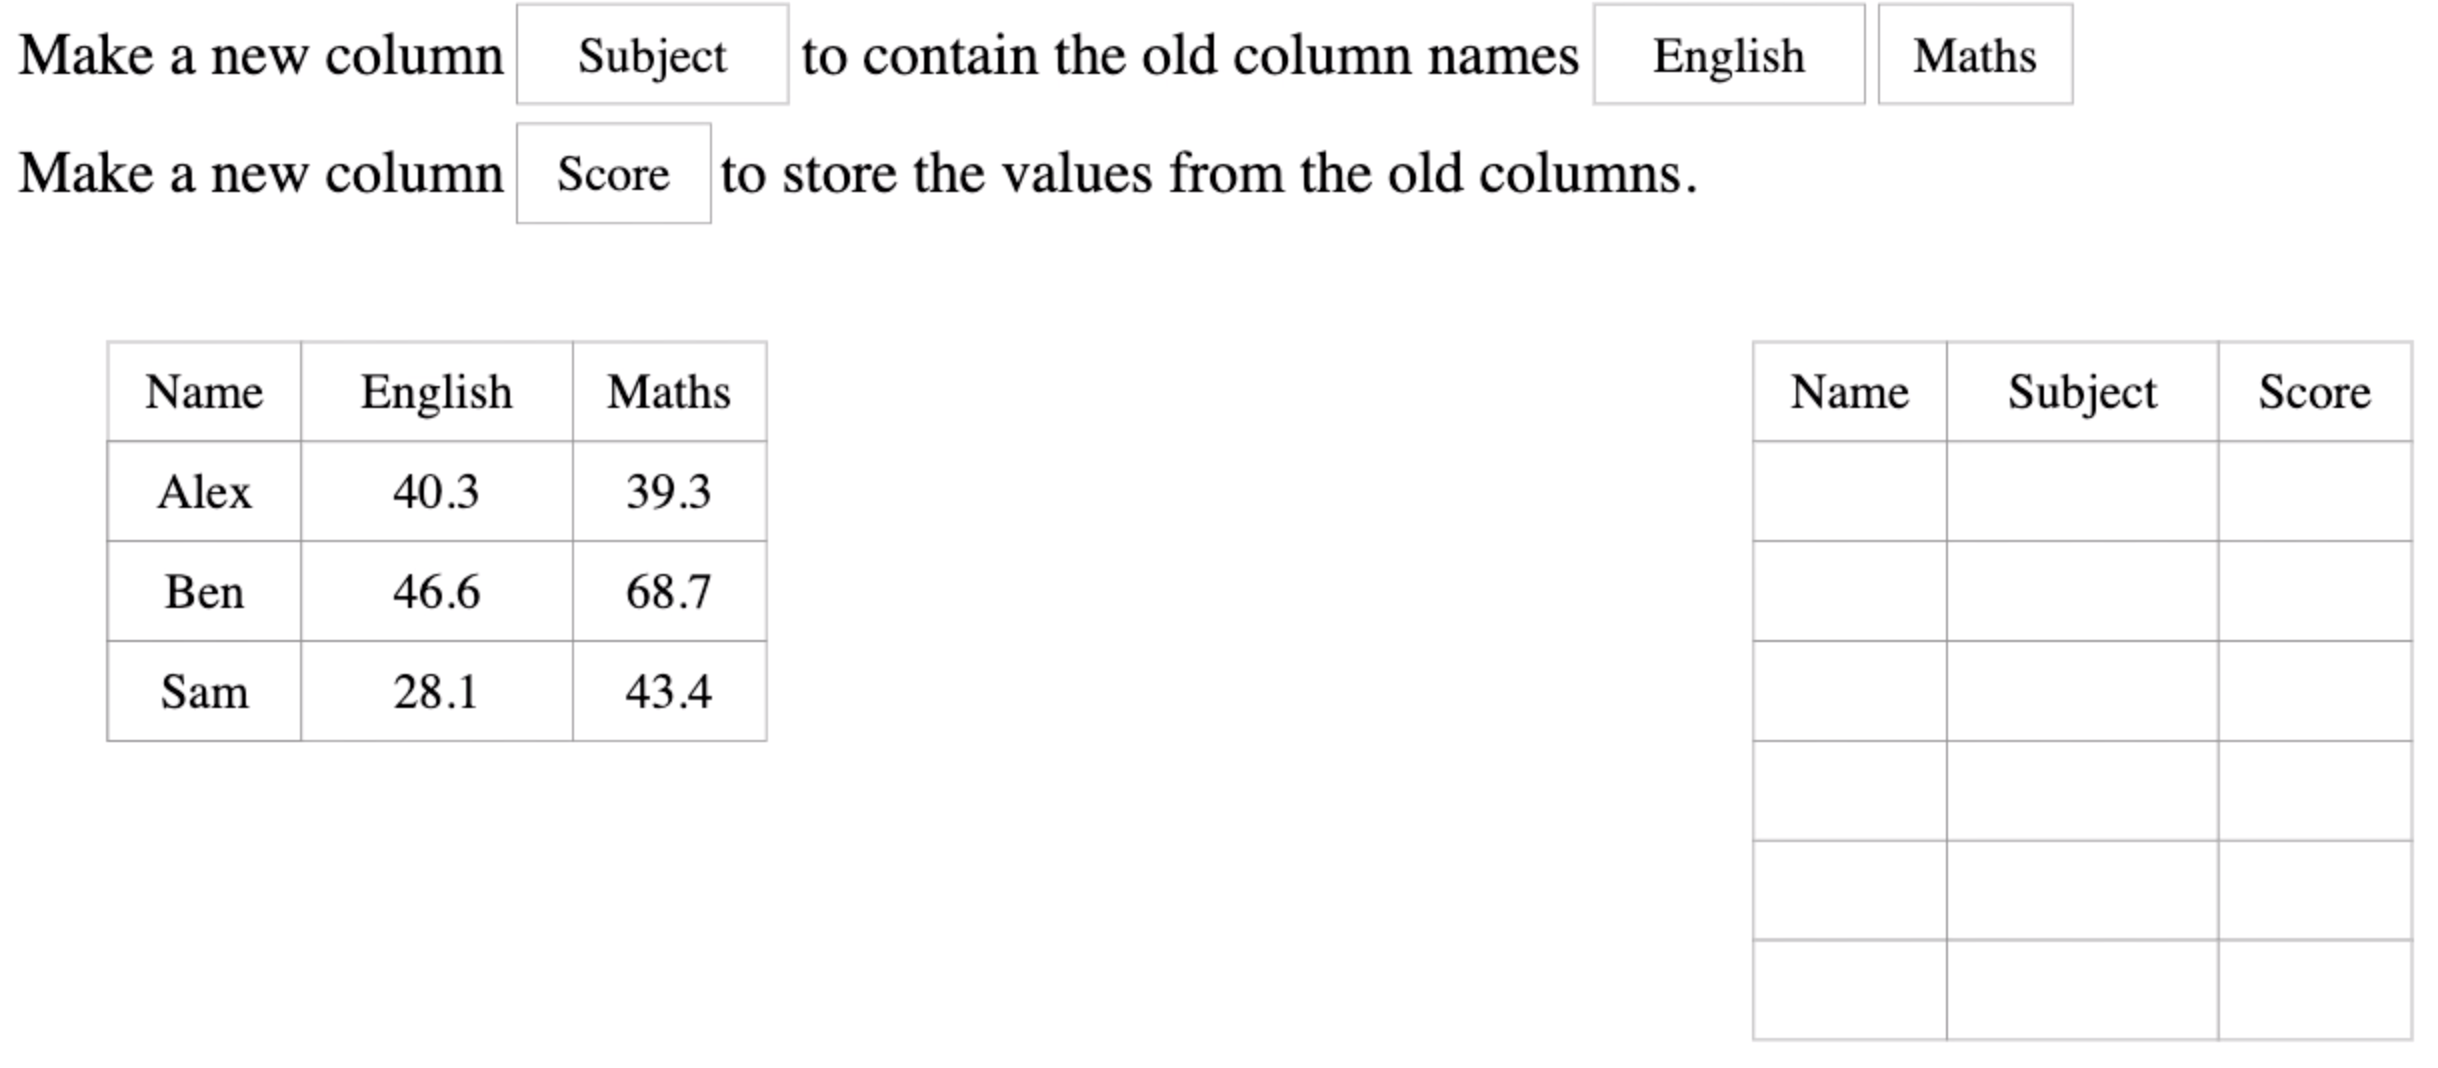
\includegraphics[scale = 0.35]{Masters-Thesis/img/gather3.png}
    \caption{Wide to Long step 3}
    \label{fig:gather3}
\end{figure}

Fourth, we fade out the tables and the text in the background and show a message informing the user that the animation will now start (Fig.~\ref{fig:gather4}). For example, here we show a message "Start wide to long transformation". We fade out the background to allow the user to focus on this message.
\begin{figure}[H]
    % \centering
    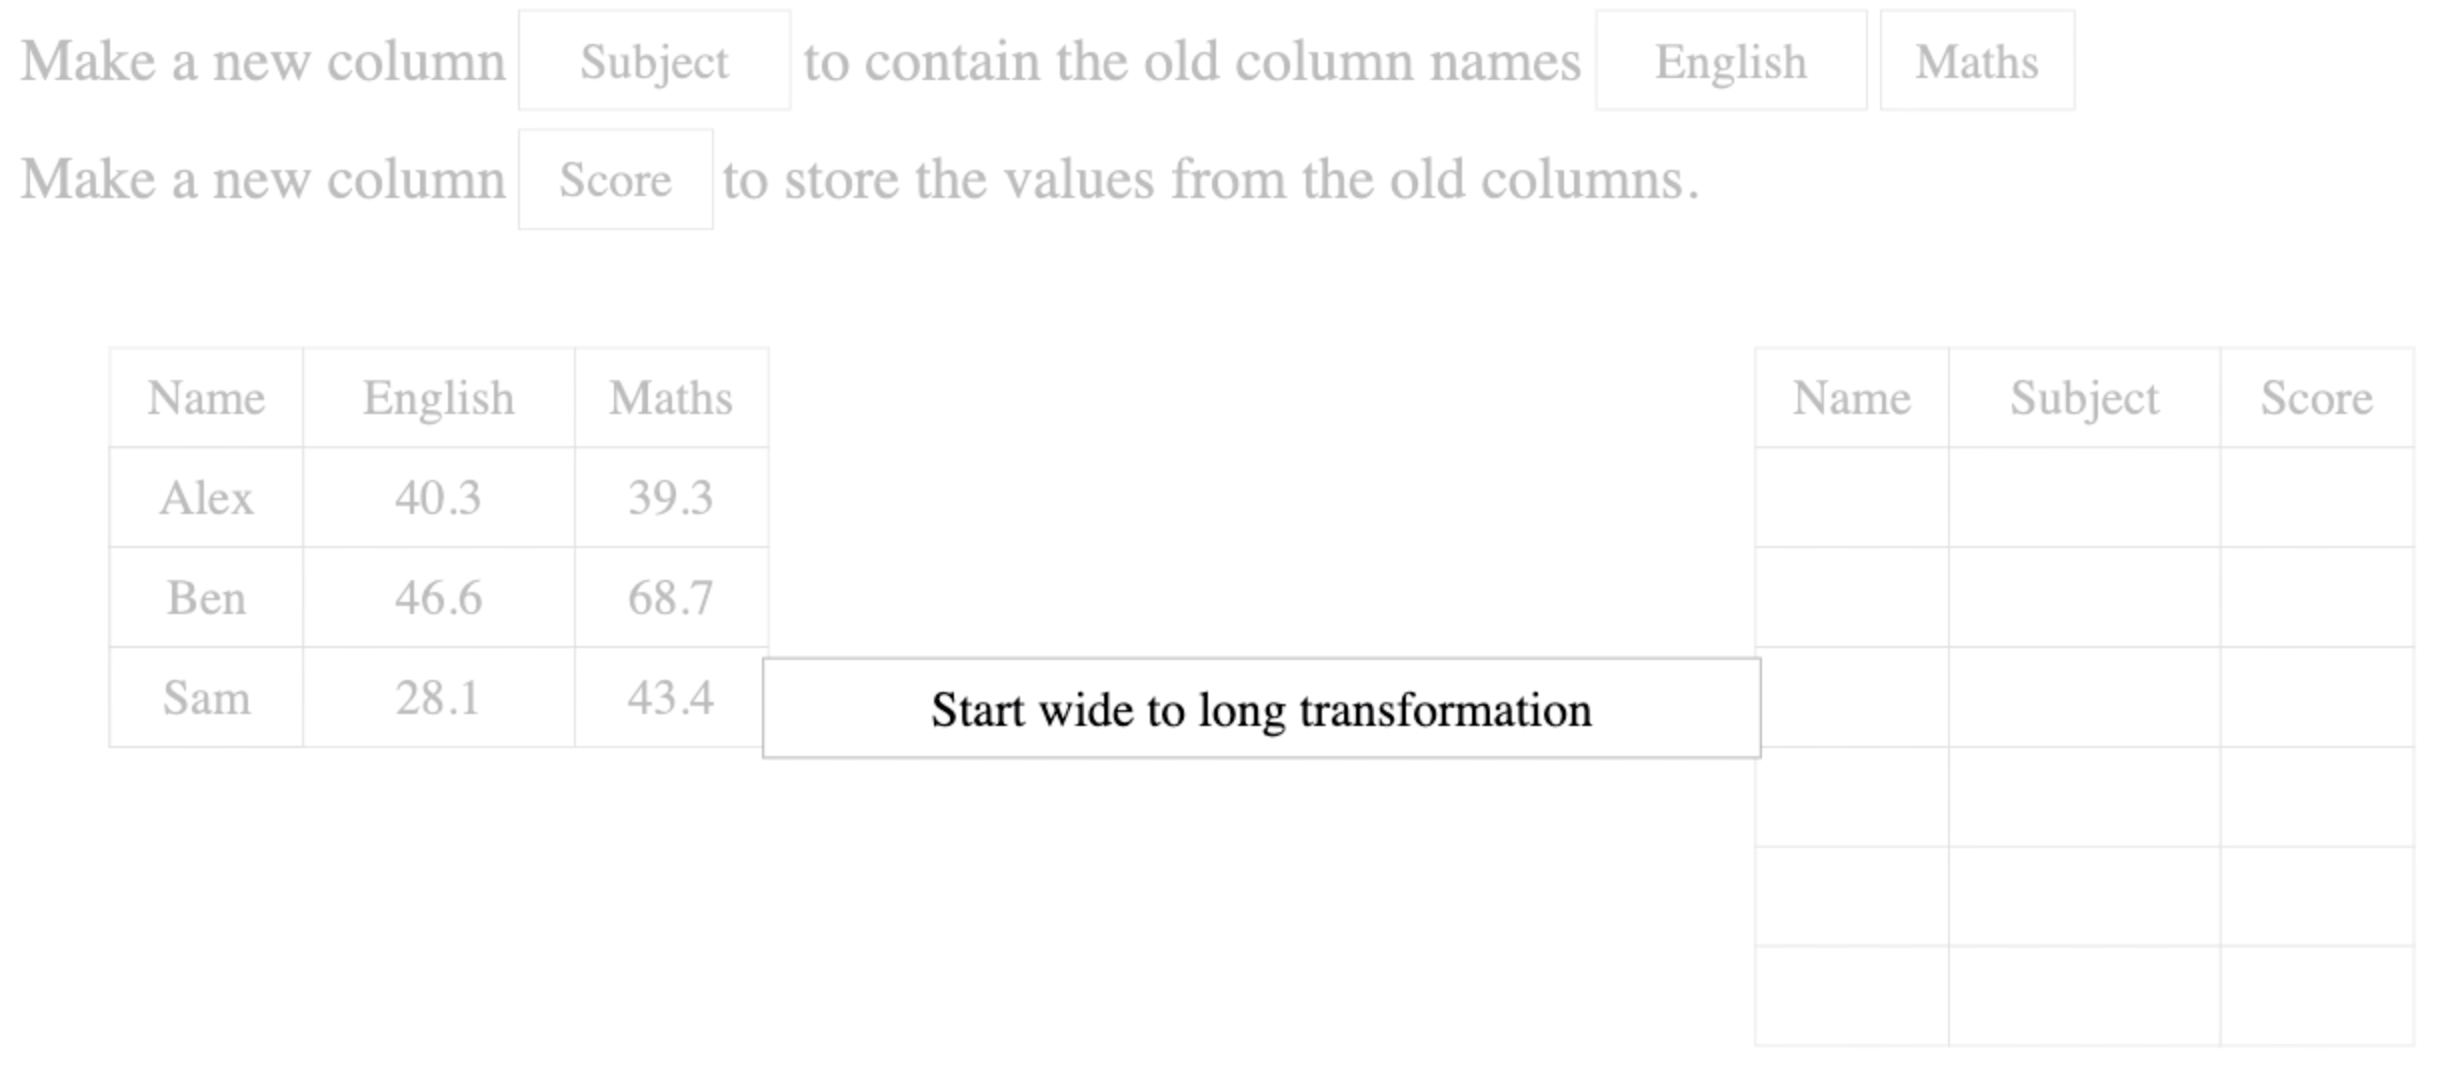
\includegraphics[scale = 0.35]{Masters-Thesis/img/gather4.png}
    \caption{Wide to Long step 4}
    \label{fig:gather4}
\end{figure}

\newpage
Fifth, we flash the column that is neither the key or the value column from both tables and link them with a line. We do this to catch the users attention.
\begin{figure}[H]
    % \centering
    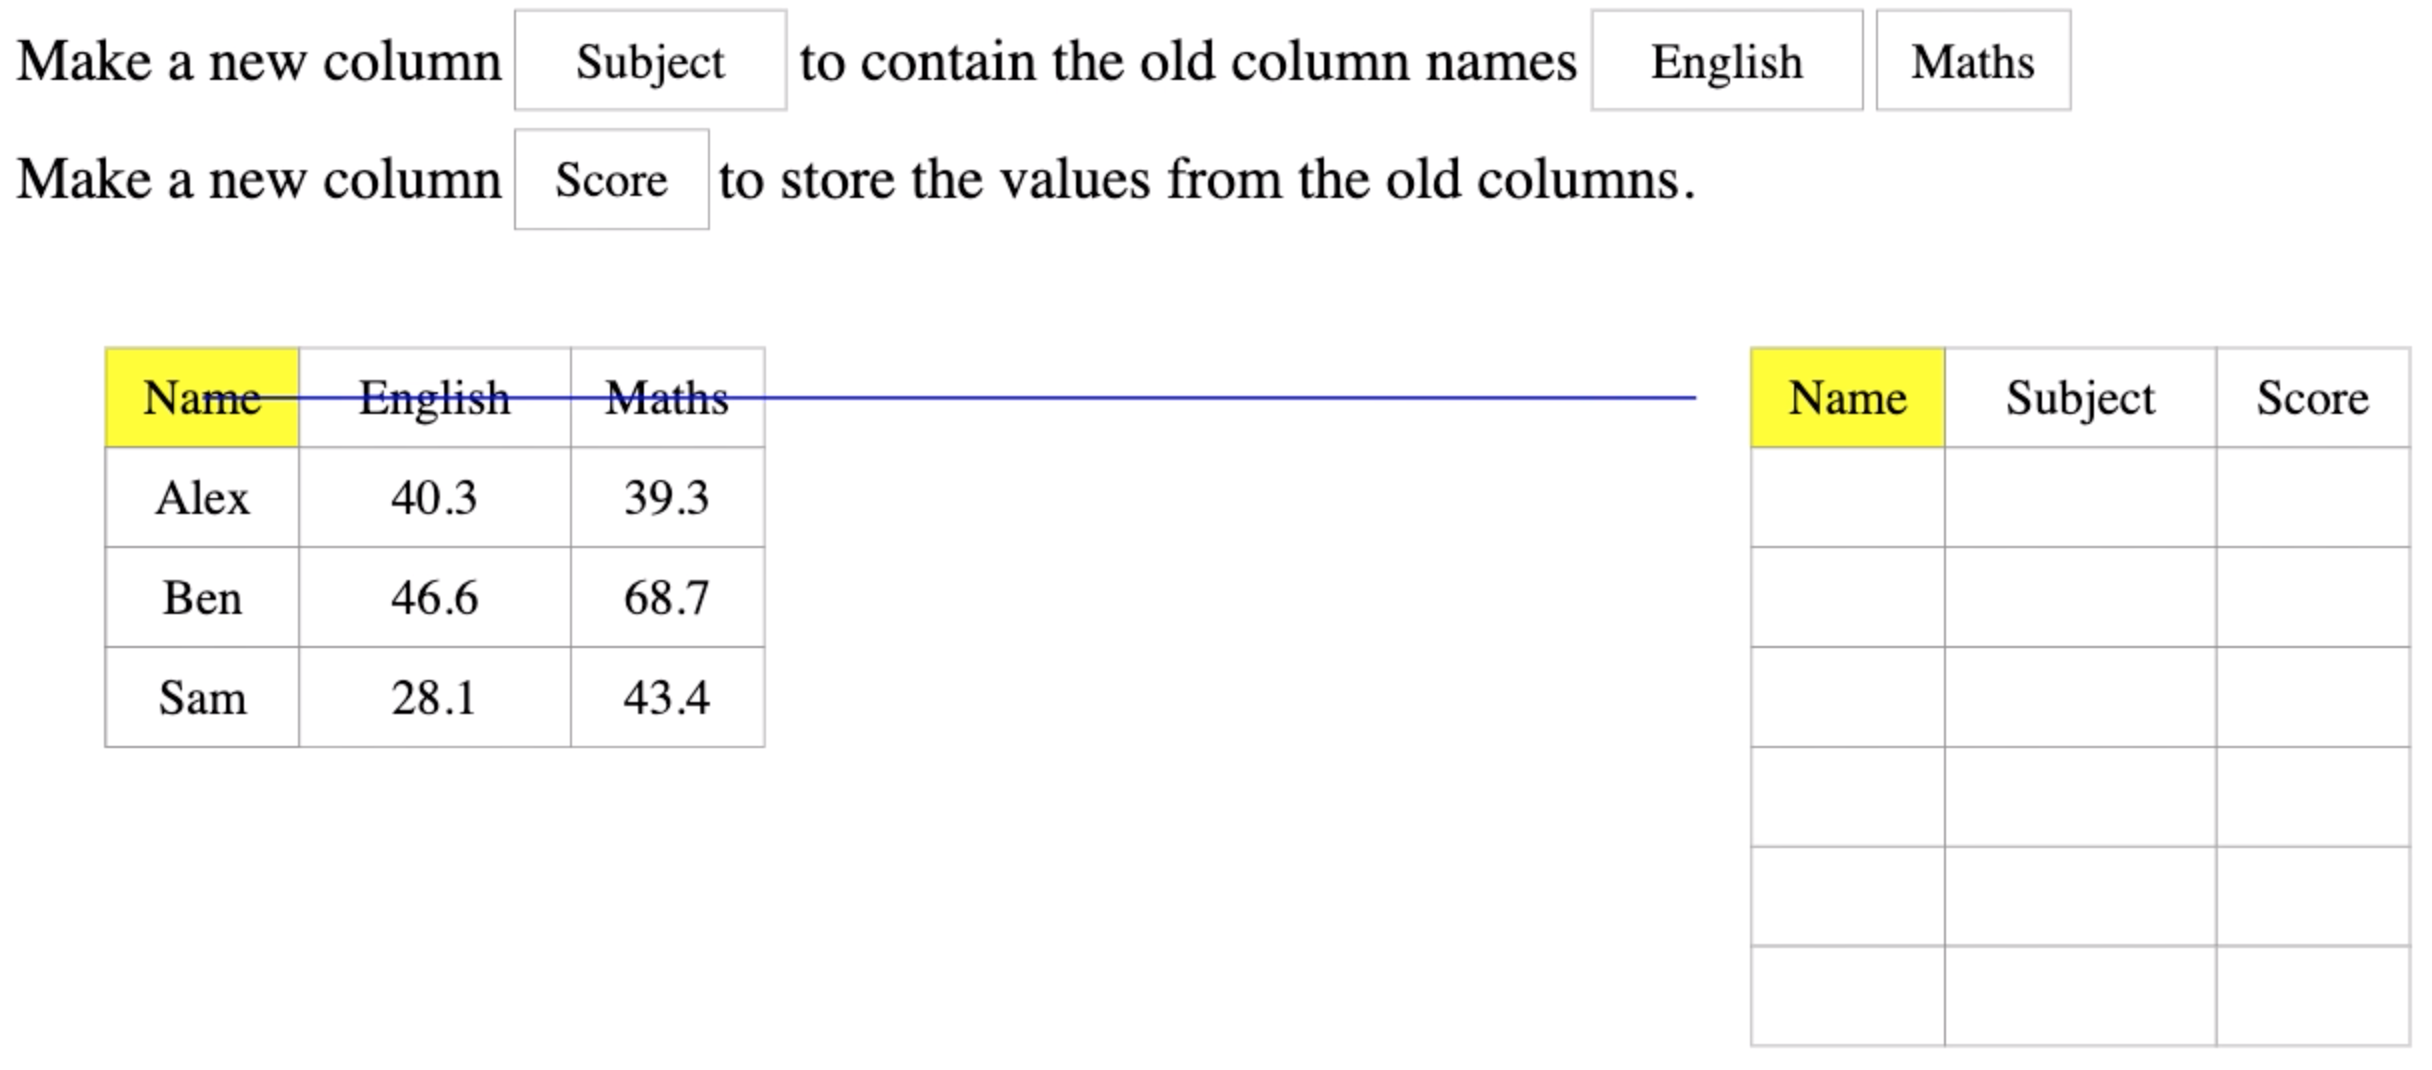
\includegraphics[scale = 0.35]{Masters-Thesis/img/gather5.png}
    \caption{Wide to Long step 5}
    \label{fig:gather5}
\end{figure}

Sixth, all the values in that column will move over to the resulted table under the same column name (Fig.~\ref{fig:gather6}, caught mid-move).
\begin{figure}[H]
    % \centering
    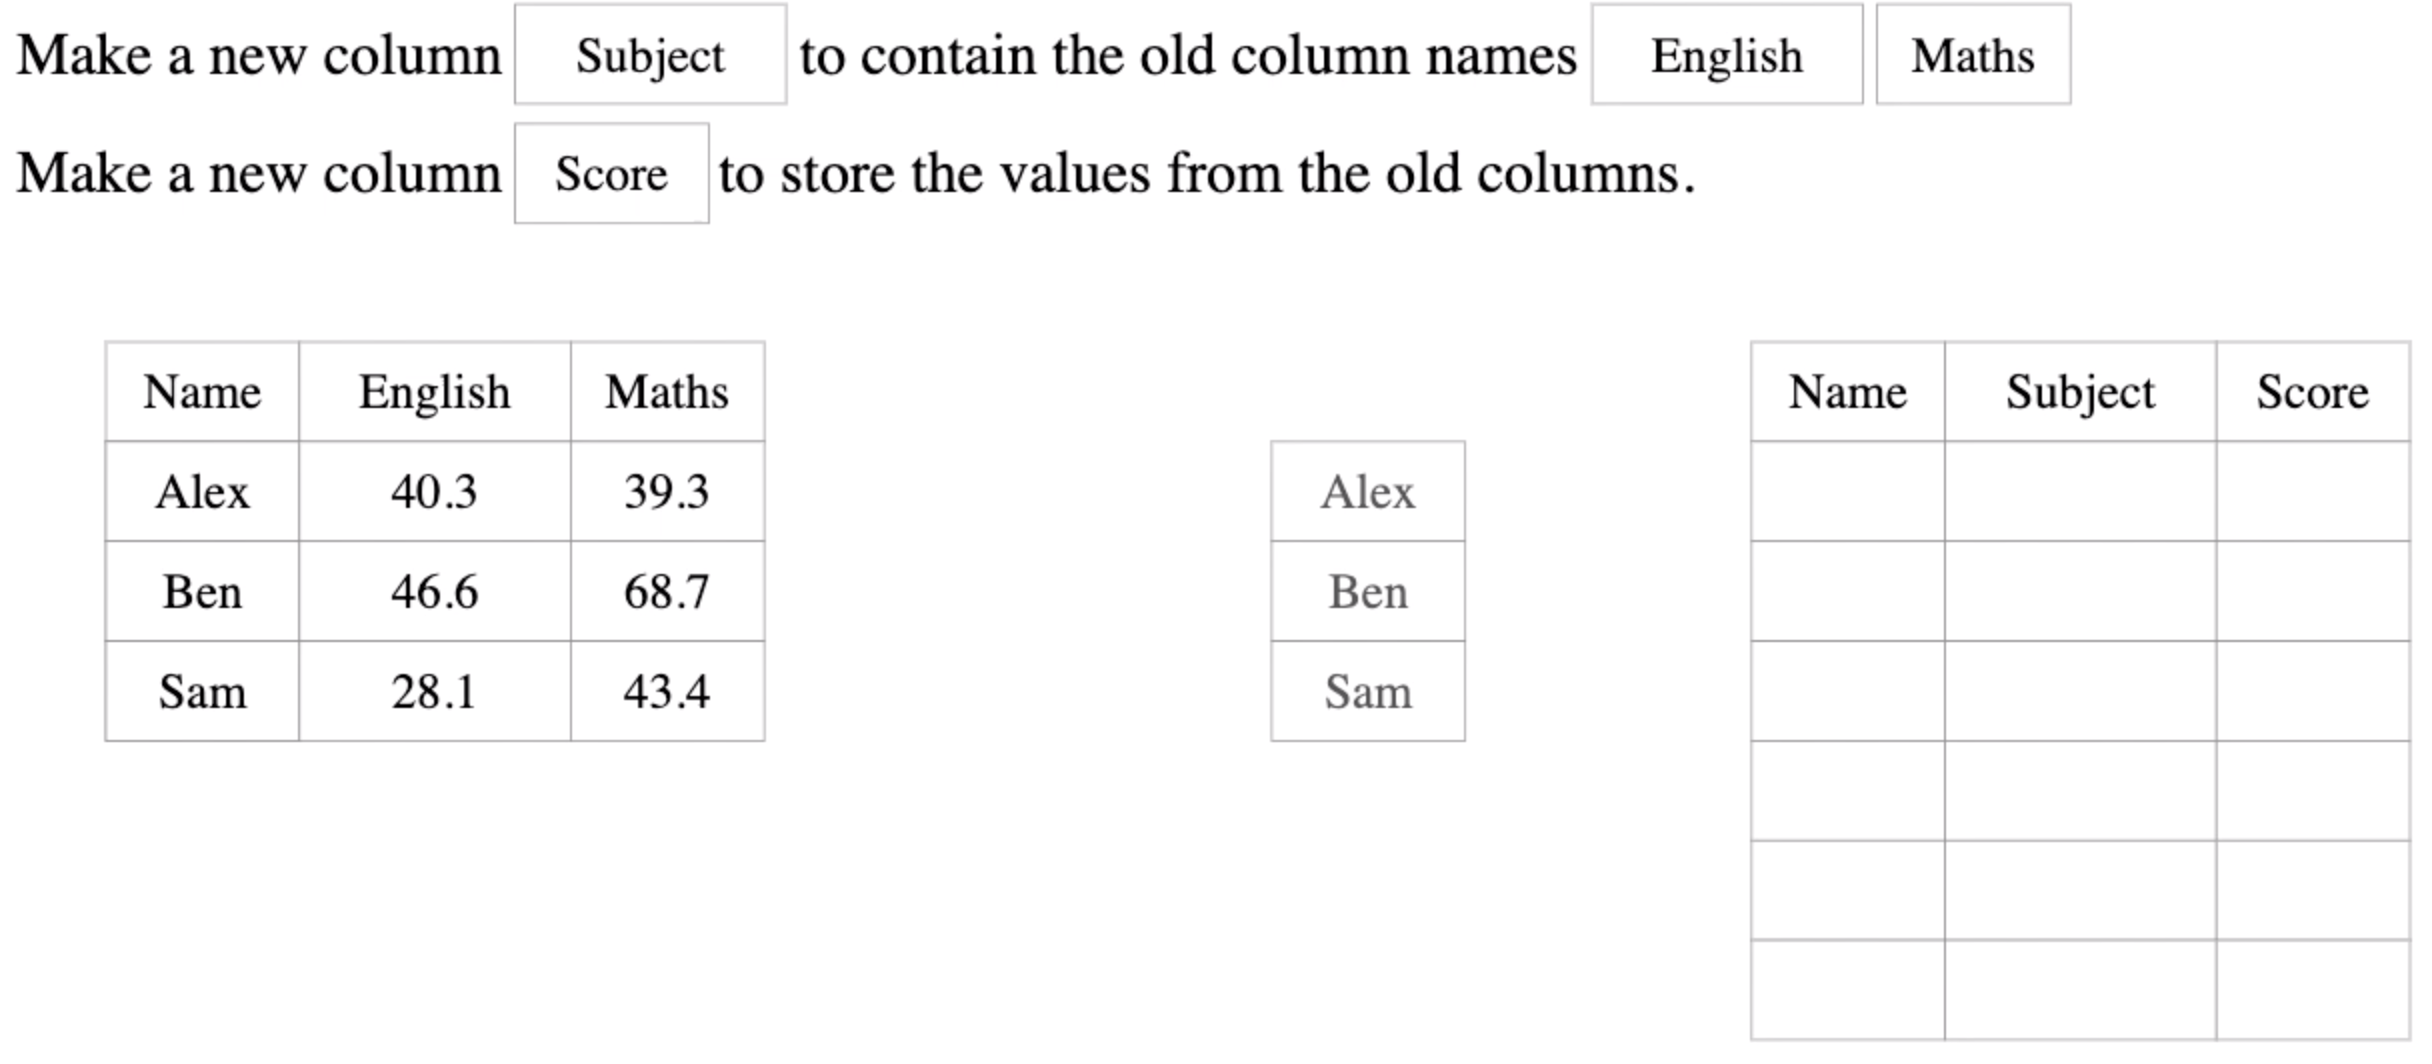
\includegraphics[scale = 0.35]{Masters-Thesis/img/gather6.png}
    \caption{Wide to Long step 6}
    \label{fig:gather6}
\end{figure}

\newpage
Seventh, we show a message informing the user that the column name of the first column which contains the values we wish to reshape will now move over to the result table under the column they specified (key) (Fig.~\ref{fig:gather7}).
\begin{figure}[H]
    % \centering
    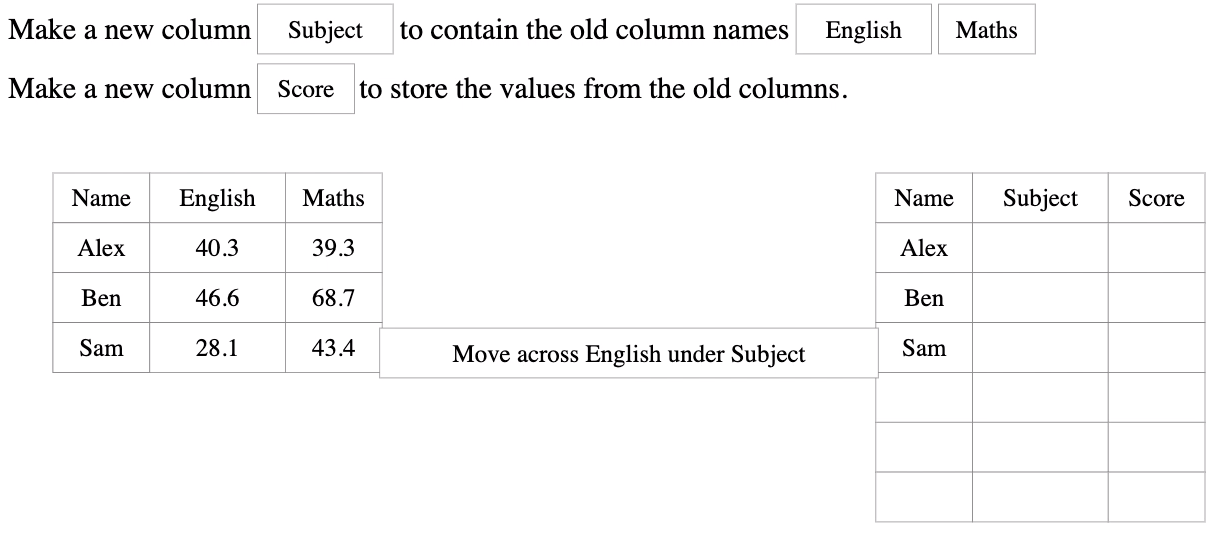
\includegraphics[scale = 0.35]{Masters-Thesis/img/gather7.png}
    \caption{Wide to Long step 7}
    \label{fig:gather7}
\end{figure}

Here the we flash the column name which we are currently animating. We also flash the corresponding location of where this element should go to further emphasise this process. Lastly, we animate lines to link these flashing elements to catch the users attention (Fig.~\ref{fig:gather8}). 
\begin{figure}[H]
    % \centering
    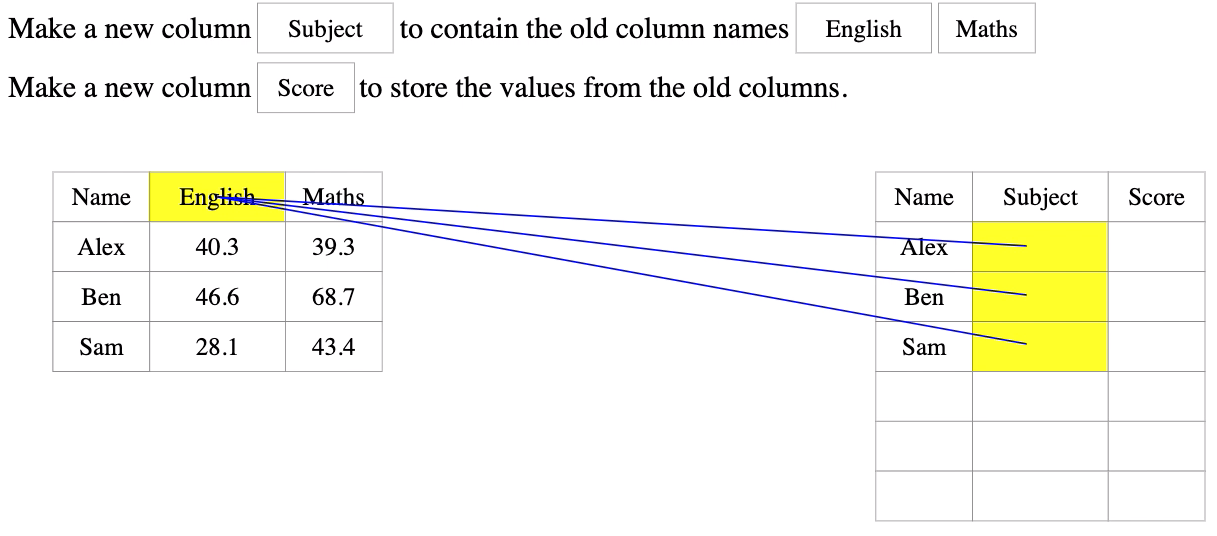
\includegraphics[scale = 0.35]{Masters-Thesis/img/gather8.png}
    \caption{Wide to Long step 8}
    \label{fig:gather8}
\end{figure}

\newpage
Next, we will move across the previously flashed column name from the original table to the locations that flashed in resulted table (Fig.~\ref{fig:gather9}). In this example, to compensate for the multiple locations that this element needs to go, we duplicate this element. The elements may or may not duplicate itself, this depends on the structure of the table.
\begin{figure}[H]
    % \centering
    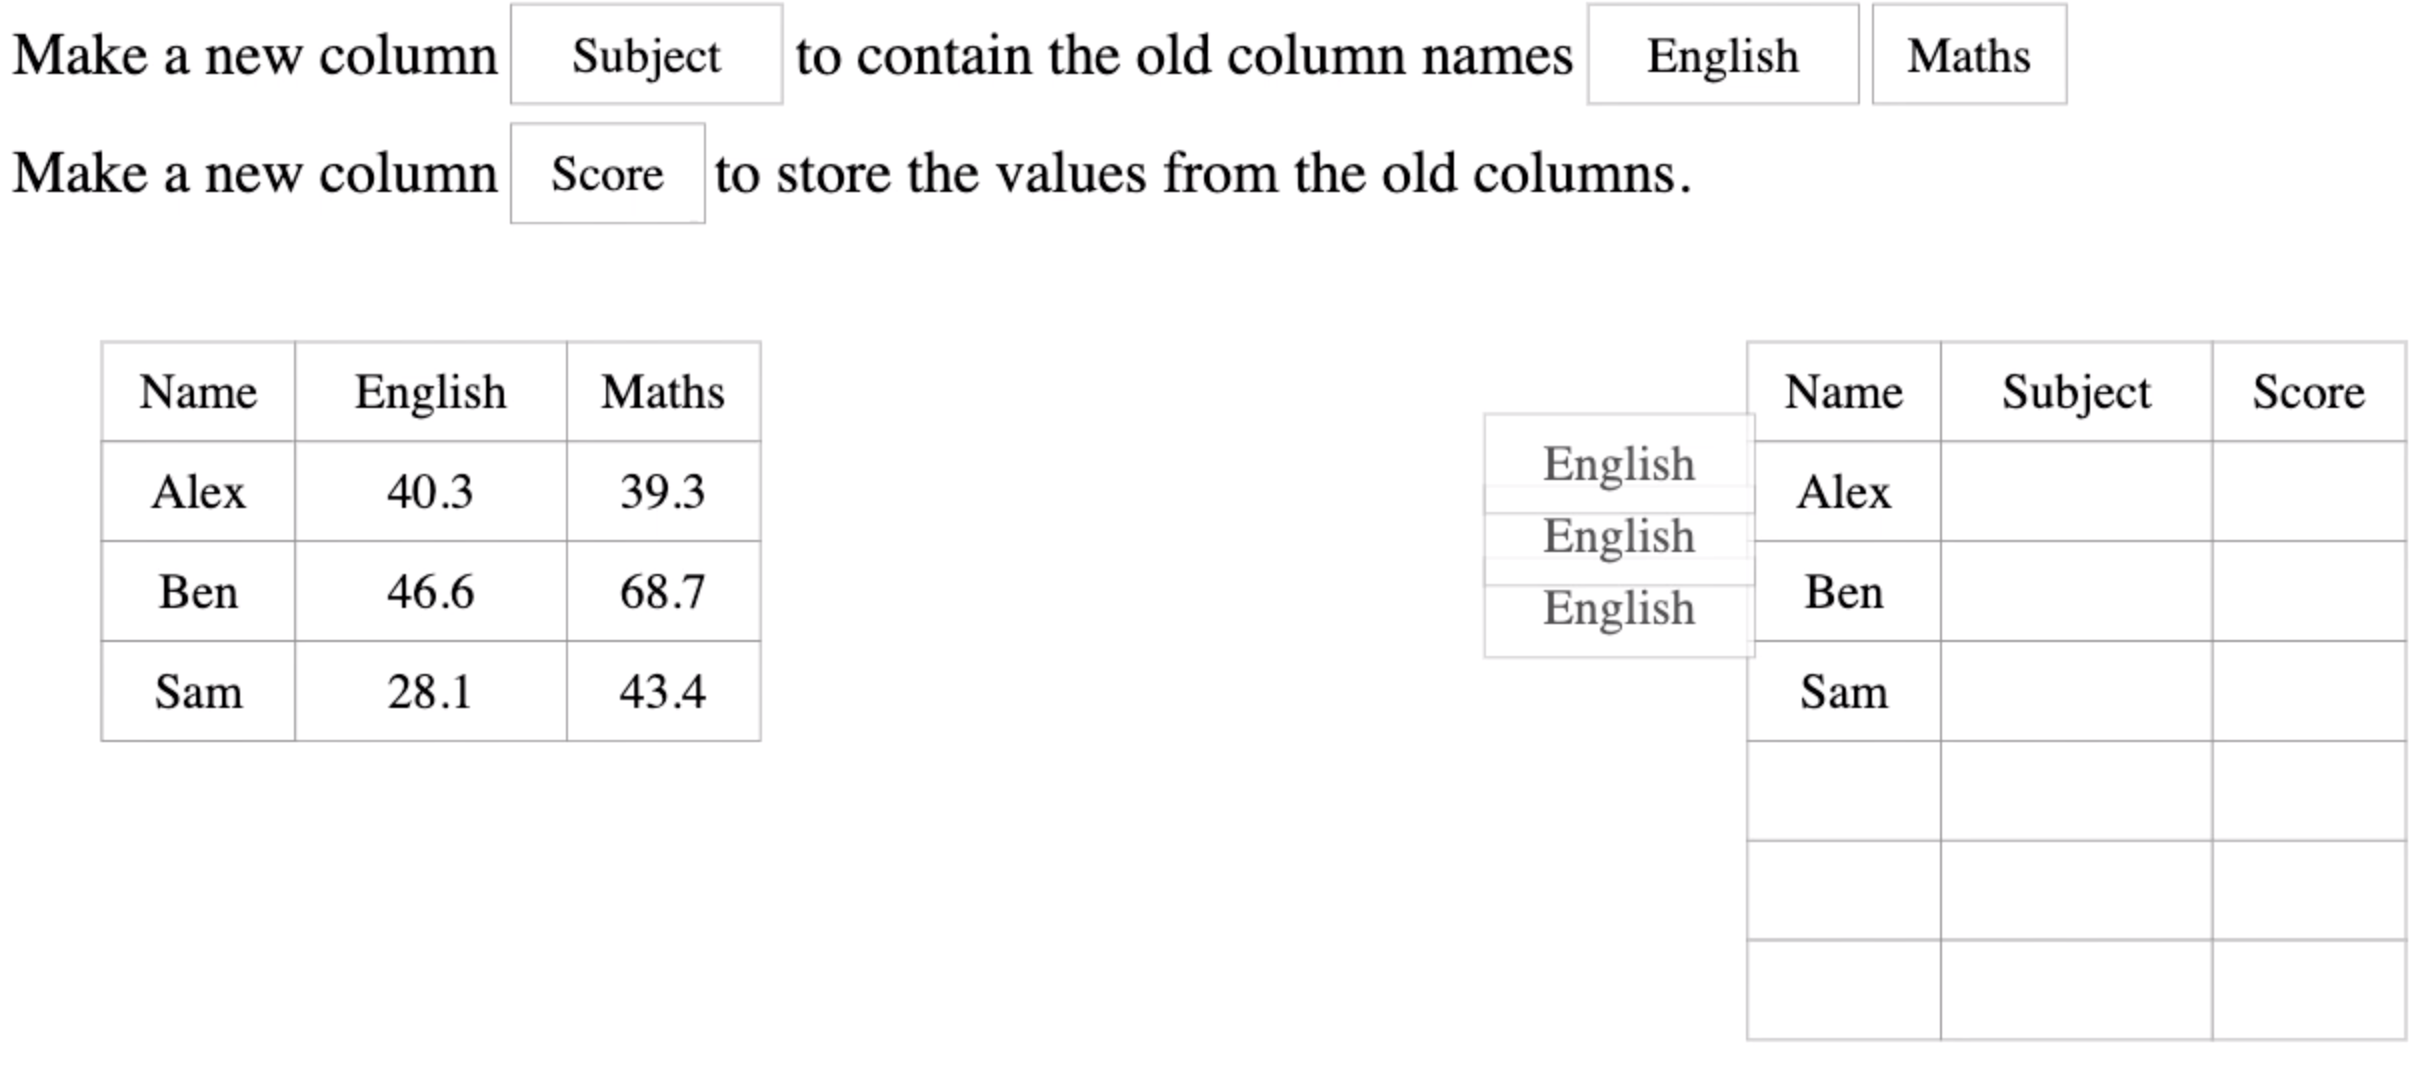
\includegraphics[scale = 0.35]{Masters-Thesis/img/gather9.png}
    \caption{Wide to Long step 9}
    \label{fig:gather9}
\end{figure}

Next, we show a message to prepare the user for the next step. The next step is to move the across corresponding values that are under the previously moved column name to the resulted table. Here they are the values under in the English column (Fig.~\ref{fig:gather10}).
\begin{figure}[H]
    % \centering
    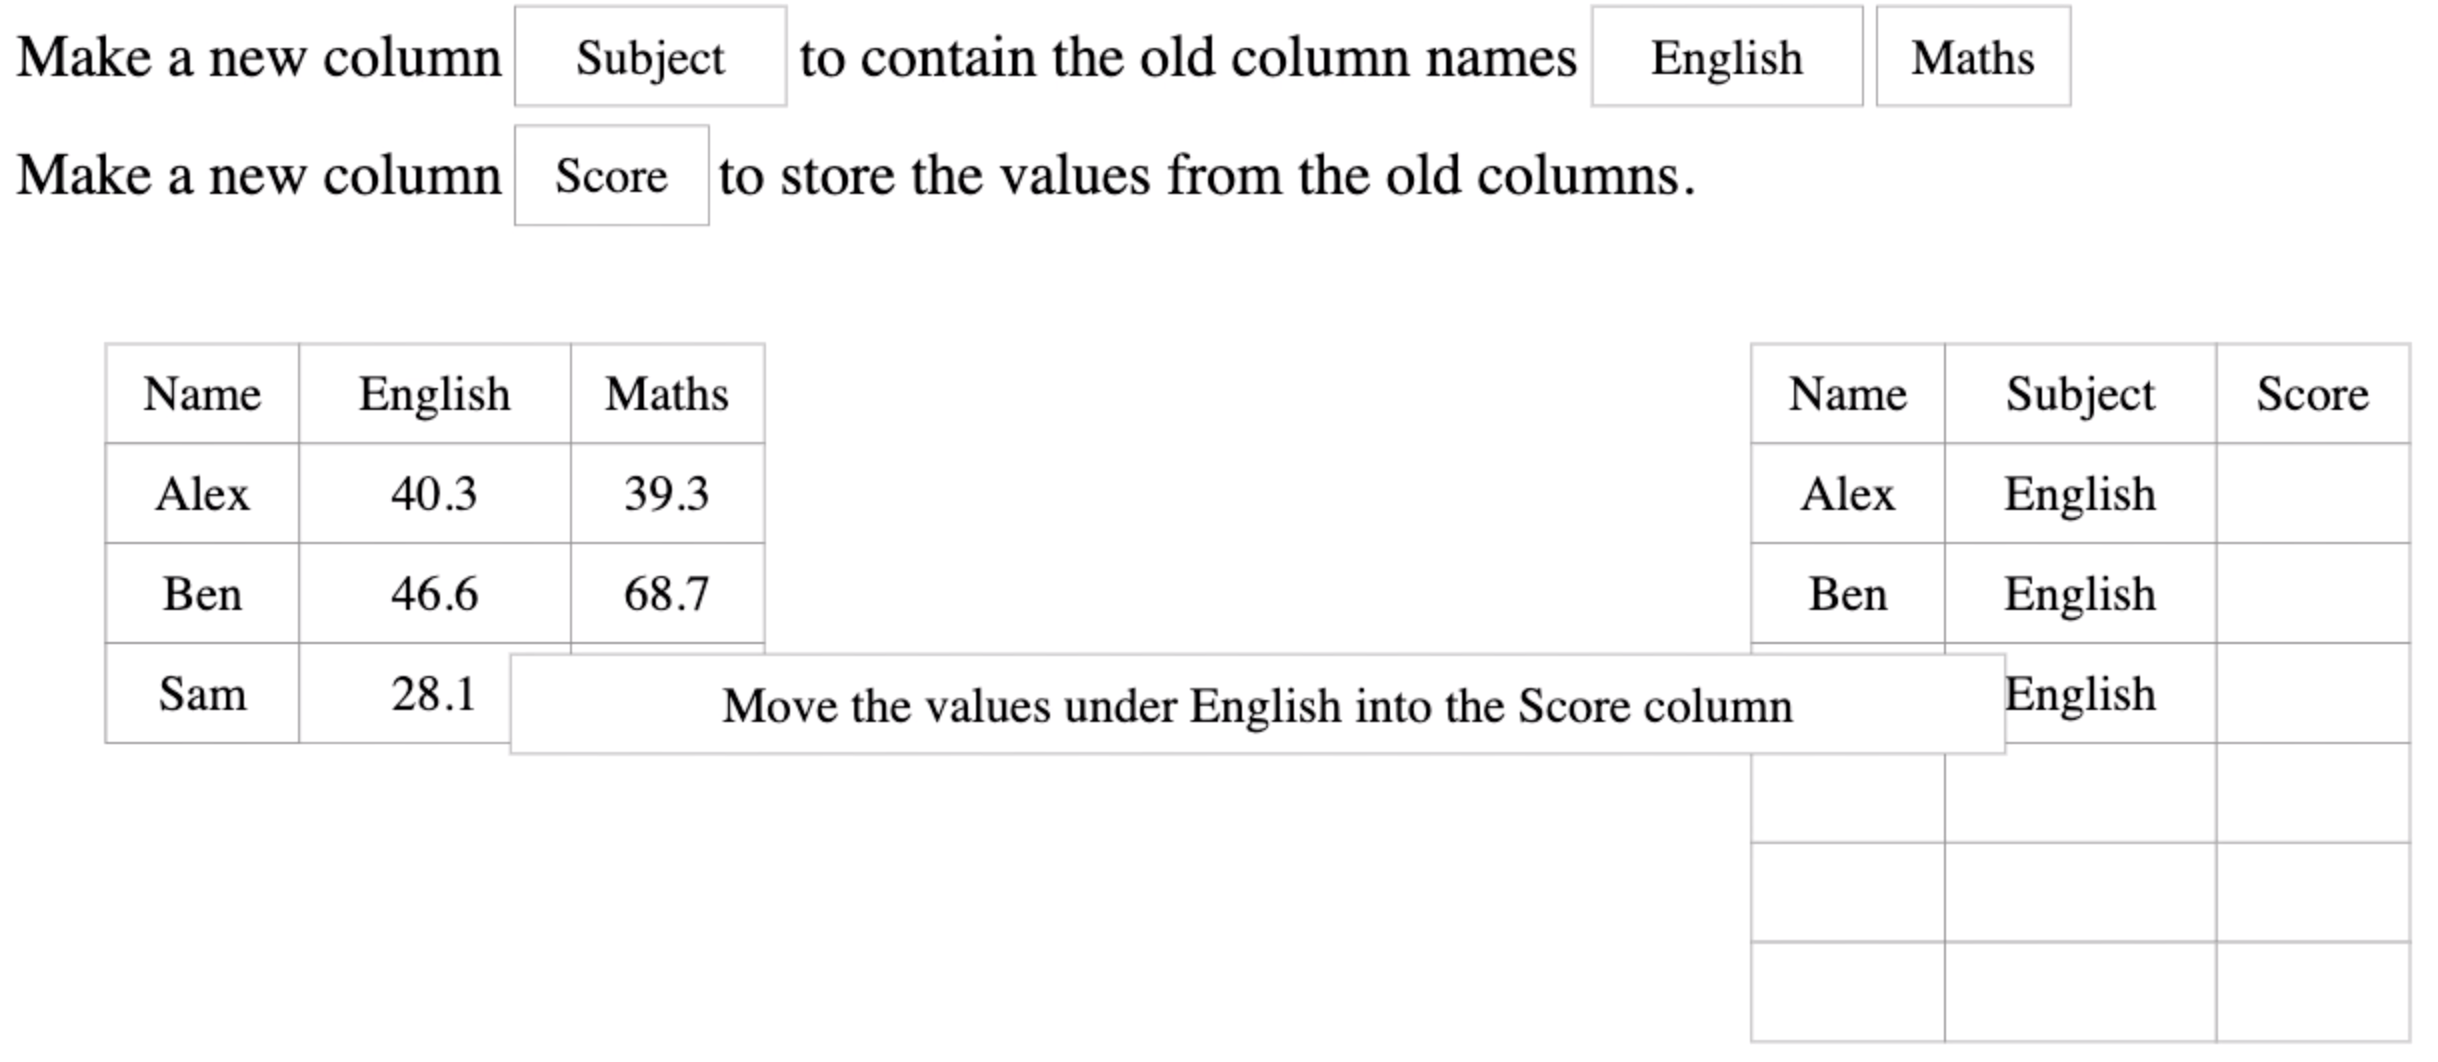
\includegraphics[scale = 0.35]{Masters-Thesis/img/gather10.png}
    \caption{Wide to Long step 10}
    \label{fig:gather10}
\end{figure}

\newpage
We then move these values across to the resulted table (Fig.~\ref{fig:gather11}, caught mid-move).
\begin{figure}[H]
    % \centering
    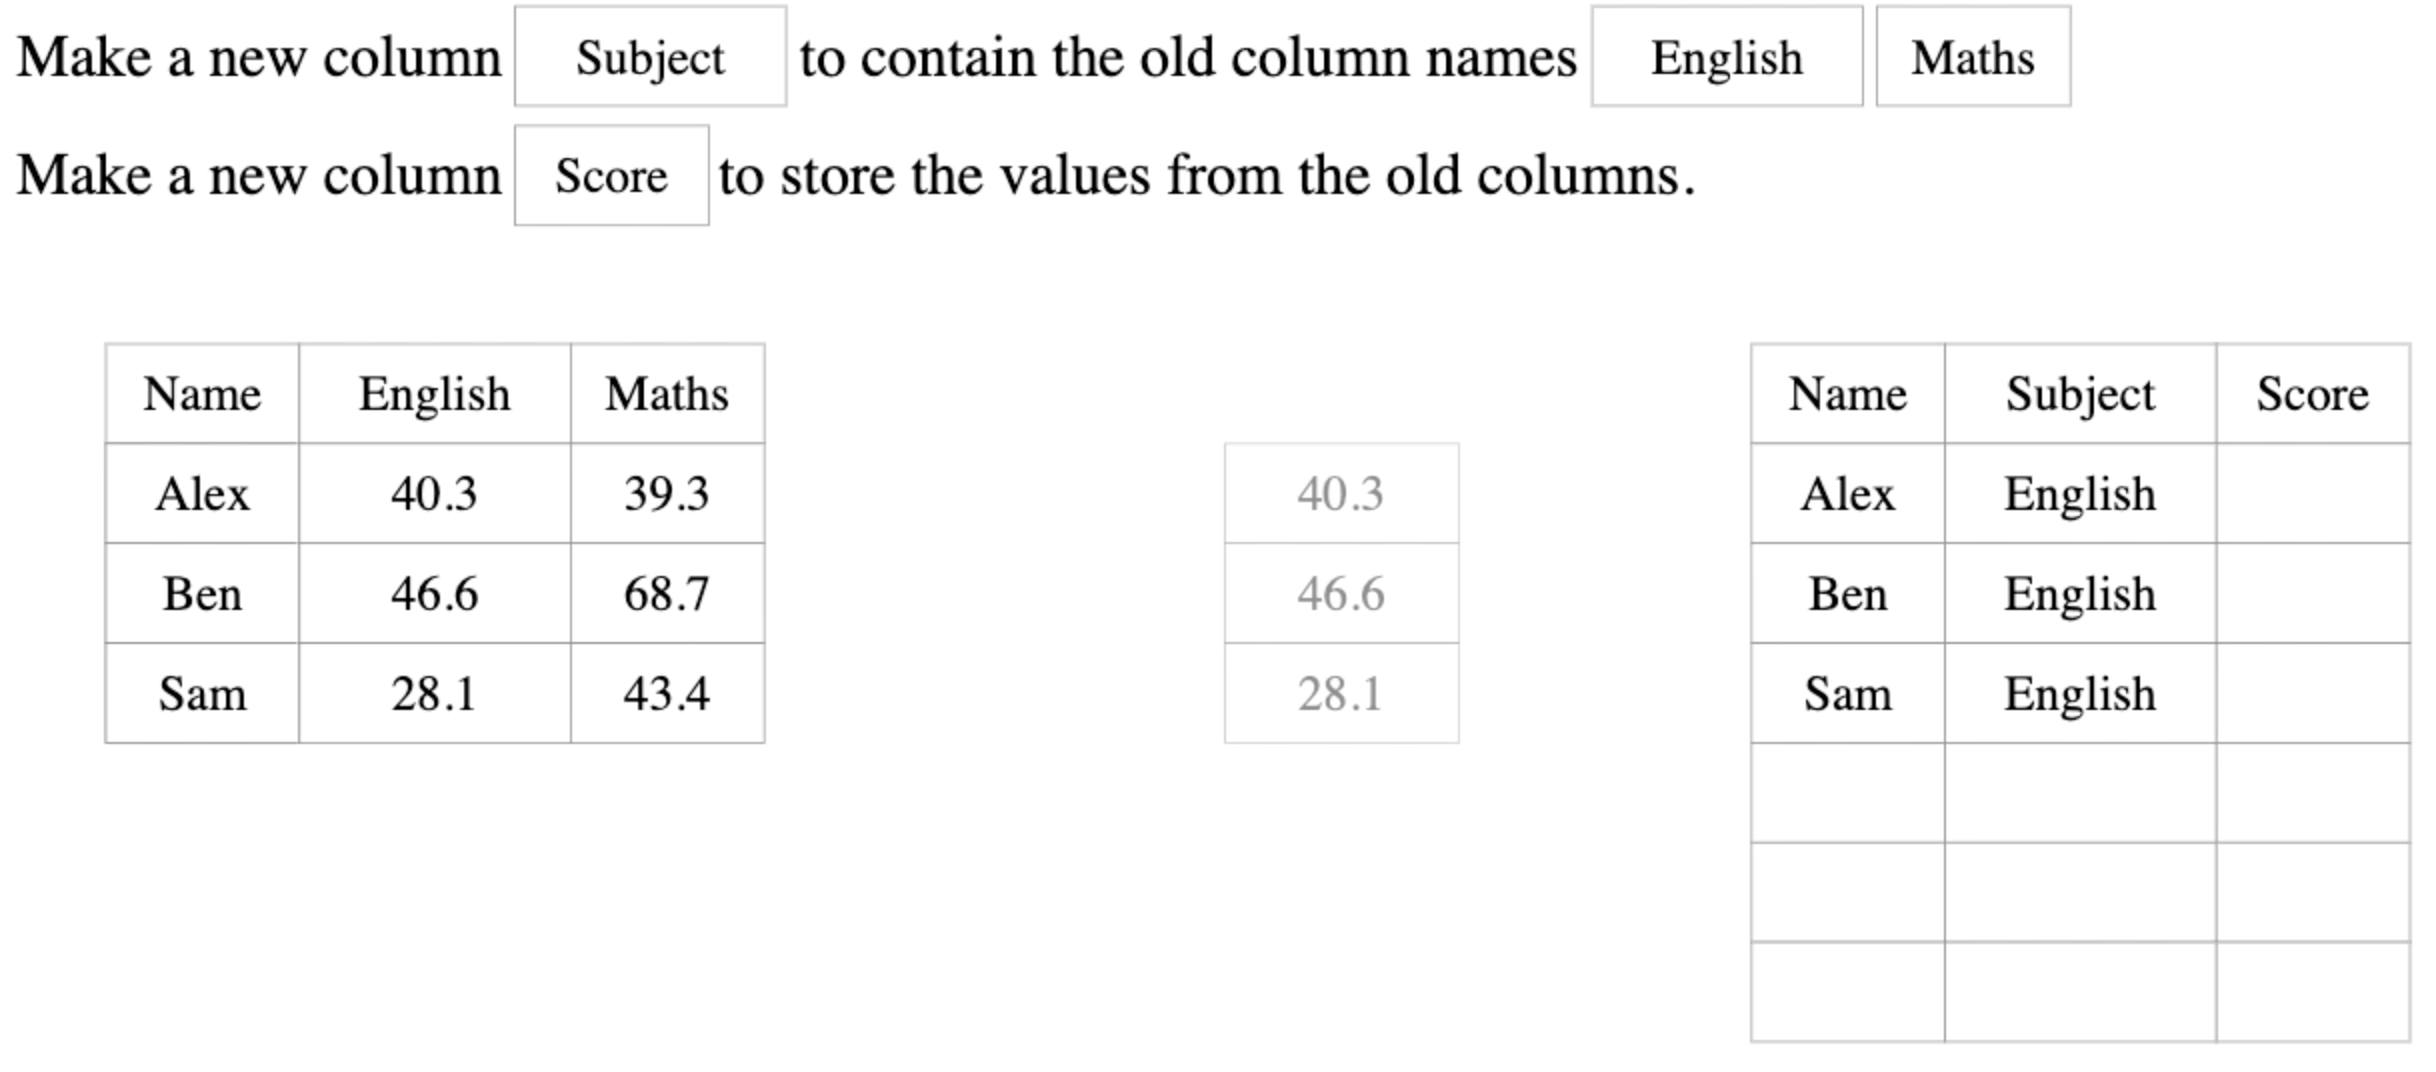
\includegraphics[scale = 0.35]{Masters-Thesis/img/gather11.png}
    \caption{Wide to Long step 11}
    \label{fig:gather11}
\end{figure}

After we finish animating the first column the user wishes to reshape on. We show a message informing the user that the animation will proceed with the next column (Fig.~\ref{fig:gather12}). In this example the next column is Maths, the process for this will be the same as the previously explained steps.
\begin{figure}[H]
    % \centering
    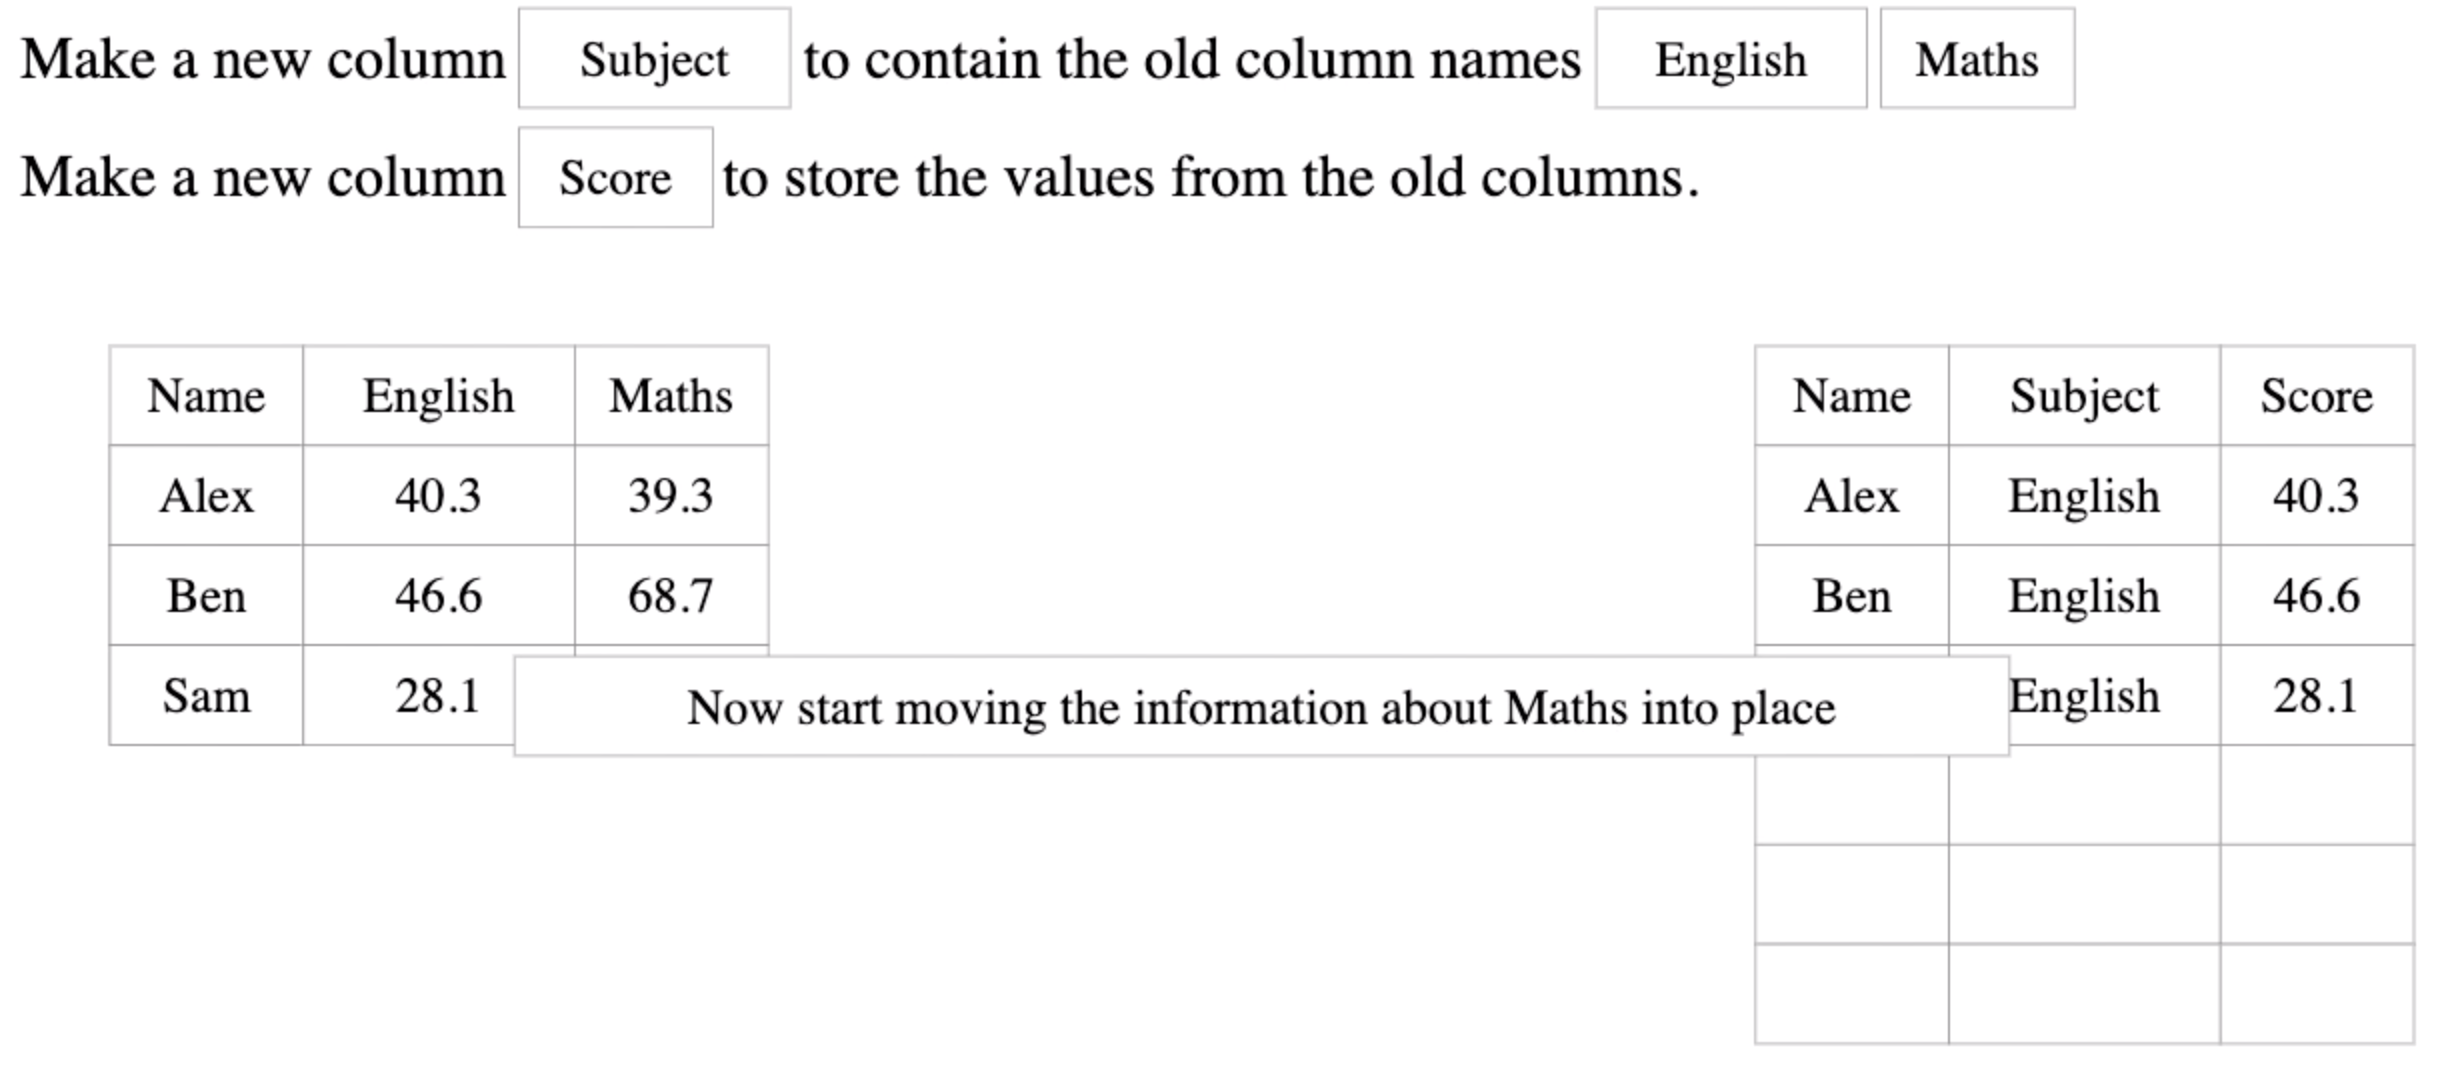
\includegraphics[scale = 0.35]{Masters-Thesis/img/gather12.png}
    \caption{Wide to Long step 12}
    \label{fig:gather12}
\end{figure}

\newpage

Lastly, when the animation finishes, the animation will stop (Fig.~\ref{fig:gather13}).

\begin{figure}[H]
    % \centering
    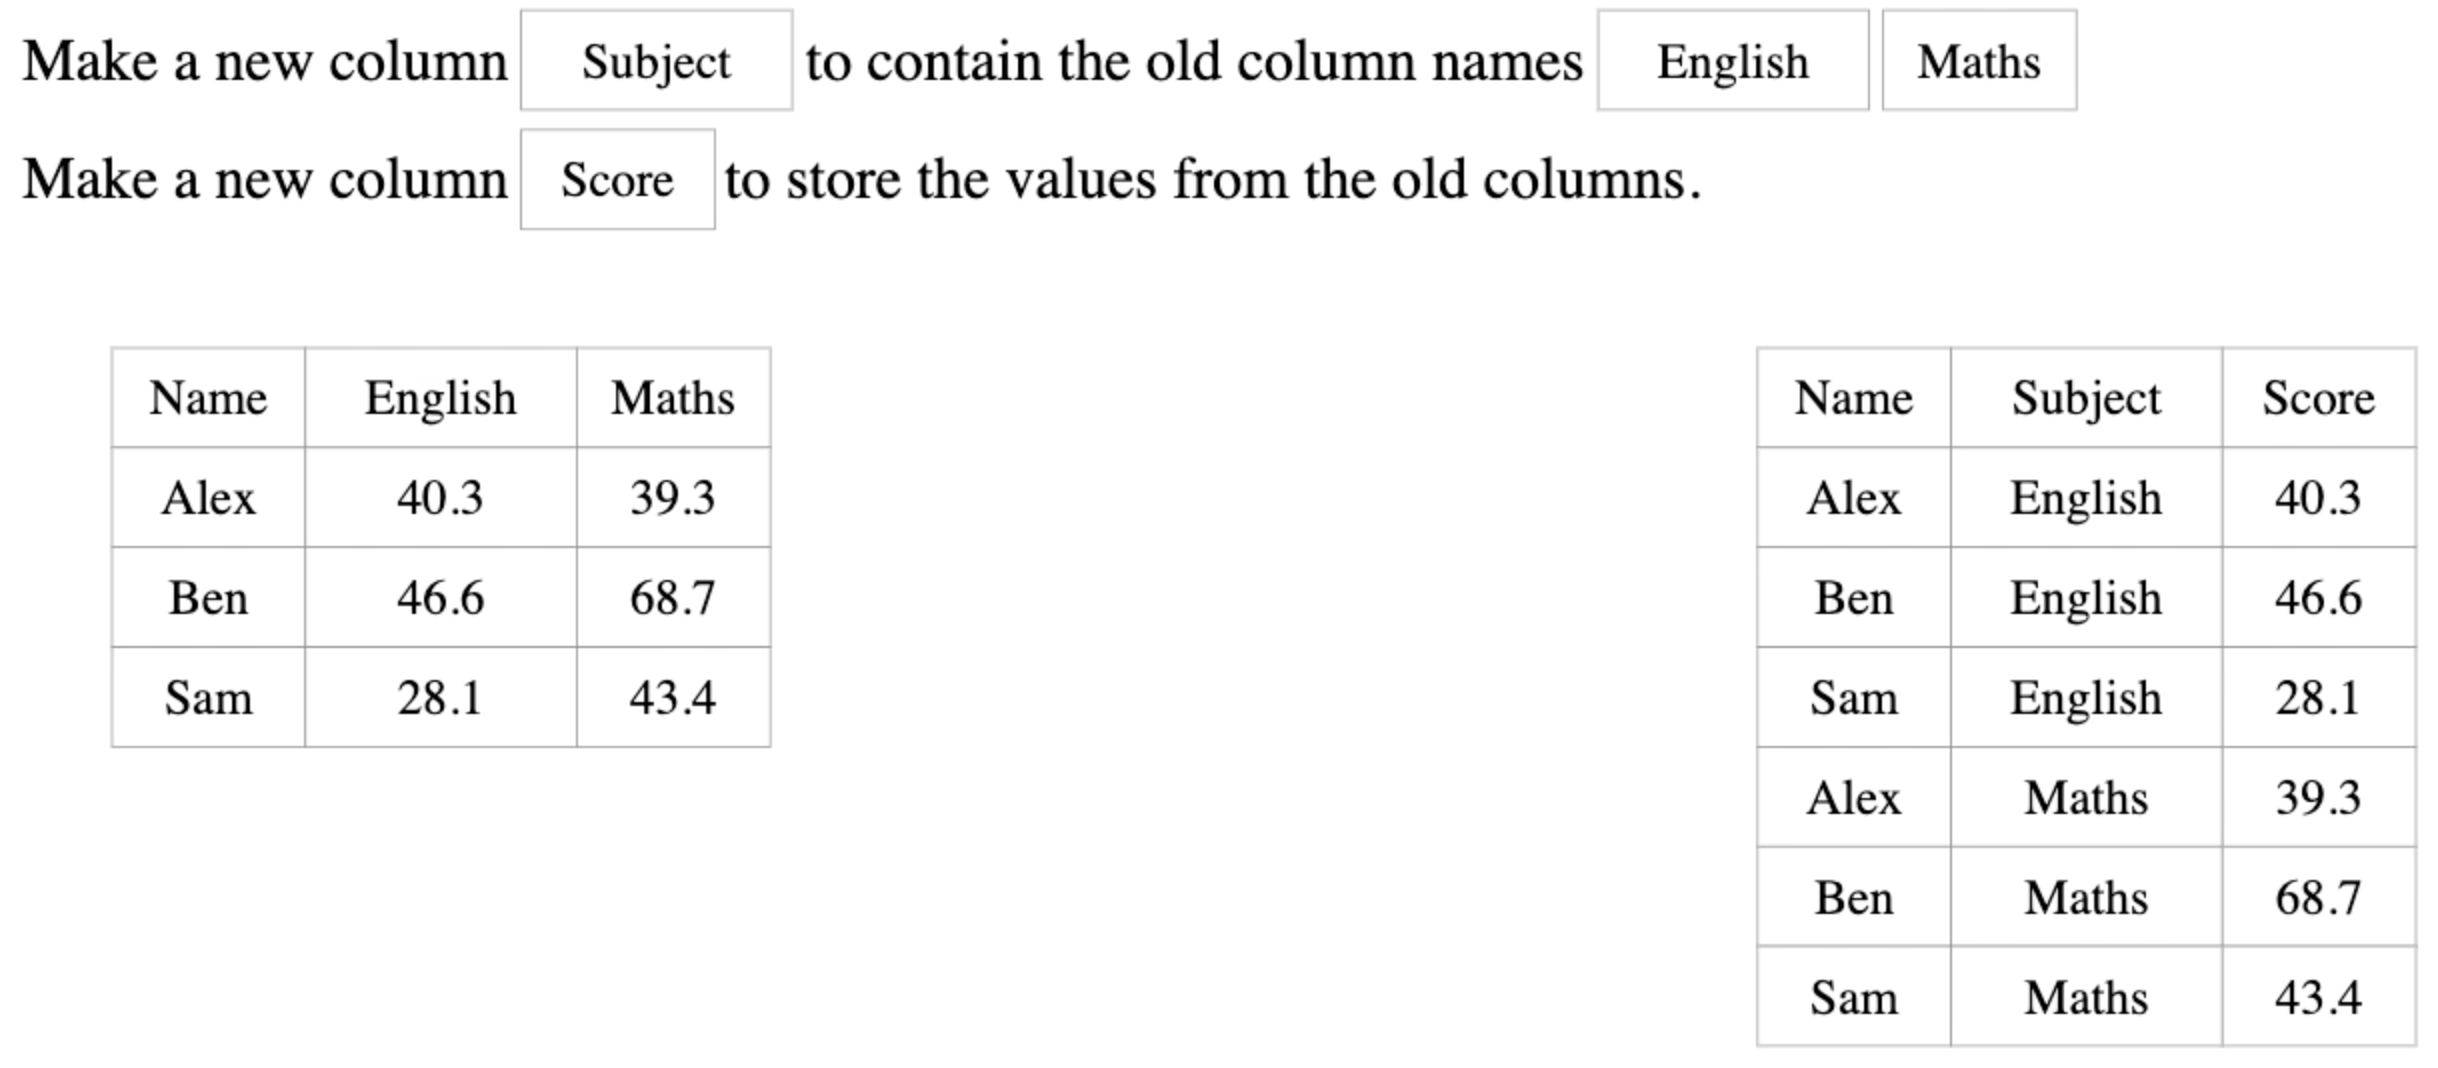
\includegraphics[scale = 0.35]{Masters-Thesis/img/gather13.png}
    \caption{Wide to Long step 13}
    \label{fig:gather13}
\end{figure}